
\documentclass[xcolor=dvipsnames]{beamer}  % for hardcopy add 'trans'

\mode<presentation>
{
  \usetheme{Singapore}
  % or ...
  \setbeamercovered{transparent}
  % or whatever (possibly just delete it)
}

\usefonttheme{professionalfonts}
\usepackage[russian]{babel}
% or whatever
%\usepackage[latin1]{inputenc}
% or whatever
%\usepackage{times}
%\usepackage[T1]{fontenc}
% Or whatever. Note that the encoding and the font should match. If T1
% does not look nice, try deleting the line with the fontenc.

%%%%%%%%%%%%%%%%%%%%%% start my preamble %%%%%%%%%%%%%%%%%%%%%%


\addtobeamertemplate{navigation symbols}{}{%
    \usebeamerfont{footline}%
    \usebeamercolor[fg]{footline}%
    \hspace{1em}%
    \insertframenumber/\inserttotalframenumber
} 

\setbeamercolor{footline}{fg=blue}
\setbeamerfont{footline}{series=\bfseries}


%\usepackage{epsfig}
\usepackage{graphicx}
\graphicspath{{./figs_code/}}

\usepackage{amsmath, amssymb, amsthm}

\usepackage{fancyvrb}

\usepackage{tikz}
\usetikzlibrary{arrows}
\usetikzlibrary{calc}
\usetikzlibrary{intersections}
\usetikzlibrary{decorations}
\usepackage{pgf}
\usepackage{pgfplots}
\pgfplotsset{compat=1.13}

\usepackage{graphviz}
 
\usepackage{verbatim}


\usepackage{algorithmicx,algpseudocode}


%font
\usepackage{mathpazo}
%\usepackage[usenames, dvipsnames]{color}

%\usepackage[linesnumbered, ruled, lined]{algorithm2e}

\usepackage{xr}
\externaldocument[ET-]{et}


\newcommand*{\theorembreak}{\usebeamertemplate{theorem end}\framebreak\usebeamertemplate{theorem begin}}

\newcommand{\newtopic}[1]{\textcolor{Green}{\Large \bf #1}}
\newcommand{\navy}[1]{\textcolor{Blue}{\bf #1}}
\newcommand{\navymth}[1]{\textcolor{Blue}{#1}}
\newcommand{\red}[1]{\textcolor{red}{#1}}


\definecolor{pale}{RGB}{235, 235, 235}
\definecolor{pale2}{RGB}{175,238,238}
\definecolor{turquois4}{RGB}{0,134,139}

% Typesetting code
\definecolor{bg}{rgb}{0.95,0.95,0.95}
\usepackage{minted}
\usemintedstyle{friendly}
\newminted{python}{mathescape,frame=lines,framesep=4mm,bgcolor=bg}
\newminted{ipython}{mathescape,frame=lines,framesep=4mm,bgcolor=bg}
\newminted{julia}{mathescape,frame=lines,framesep=4mm,bgcolor=bg}
\newminted{c}{mathescape,linenos=true}
\newminted{r}{mathescape,  frame=none, baselinestretch=1, framesep=2mm}
\renewcommand{\theFancyVerbLine}{\sffamily
    \textcolor[rgb]{0.5,0.5,1.0}{\scriptsize {\arabic{FancyVerbLine}}}}


\usepackage{stmaryrd}

\newcommand{\Fact}{\textcolor{Brown}{\bf Факт. }}
\newcommand{\Facts}{\textcolor{Brown}{\bf Факты }}
\newcommand{\keya}{\textcolor{turquois4}{\bf Ключевая идея. }}
\newcommand{\Factnodot}{\textcolor{Brown}{\bf Факт }}
\newcommand{\Eg}{\textcolor{ForestGreen}{Пример. }}
\newcommand{\Egs}{\textcolor{ForestGreen}{Примеры. }}
\newcommand{\Ex}{{\bf Ex. }}
\newcommand{\Thm}{\textcolor{Brown}{\bf Теорема. }}
\newcommand{\Prf}{\textcolor{turquois4}{\bf Доказательство. }}
\newcommand{\Ass}{\textcolor{turquois4}{\bf Допущение.}} 
\newcommand{\Lem}{\textcolor{Brown}{\bf Лемма. }}

%source code 



% cali
\usepackage{mathrsfs}
\usepackage{bbm}
\usepackage{subfigure}

\newcommand{\argmax}{\operatornamewithlimits{argmax}}
\newcommand{\argmin}{\operatornamewithlimits{argmin}}

\newcommand\T{{\mathpalette\raiseT\intercal}}
\newcommand\raiseT[2]{\raisebox{0.25ex}{$#1#2$}}

\DeclareMathOperator{\cl}{cl}
%\DeclareMathOperator{\argmax}{argmax}
\DeclareMathOperator{\interior}{int}
\DeclareMathOperator{\Prob}{Prob}
\DeclareMathOperator{\kernel}{ker}
\DeclareMathOperator{\diag}{diag}
\DeclareMathOperator{\sgn}{sgn}
\DeclareMathOperator{\determinant}{det}
\DeclareMathOperator{\trace}{trace}
\DeclareMathOperator{\Span}{span}
\DeclareMathOperator{\rank}{rank}
\DeclareMathOperator{\cov}{cov}
\DeclareMathOperator{\corr}{corr}
\DeclareMathOperator{\range}{rng}
\DeclareMathOperator{\var}{var}
\DeclareMathOperator{\mse}{mse}
\DeclareMathOperator{\se}{se}
\DeclareMathOperator{\row}{row}
\DeclareMathOperator{\col}{col}
\DeclareMathOperator{\dimension}{dim}
\DeclareMathOperator{\fracpart}{frac}
\DeclareMathOperator{\proj}{proj}
\DeclareMathOperator{\colspace}{colspace}

\providecommand{\inner}[1]{\left\langle{#1}\right\rangle}

% mics short cuts and symbols
% mics short cuts and symbols
\newcommand{\st}{\ensuremath{\ \mathrm{s.t.}\ }}
\newcommand{\setntn}[2]{ \{ #1 : #2 \} }
\newcommand{\cf}[1]{ \lstinline|#1| }
\newcommand{\otms}[1]{ \leftidx{^\circ}{#1}}

\newcommand{\fore}{\therefore \quad}
\newcommand{\tod}{\stackrel { d } {\to} }
\newcommand{\tow}{\stackrel { w } {\to} }
\newcommand{\toprob}{\stackrel { p } {\to} }
\newcommand{\toms}{\stackrel { ms } {\to} }
\newcommand{\eqdist}{\stackrel {\textrm{ \scriptsize{d} }} {=} }
\newcommand{\iidsim}{\stackrel {\textrm{ {\sc iid }}} {\sim} }
\newcommand{\1}{\mathbbm 1}
\newcommand{\dee}{\,{\rm d}}
\newcommand{\given}{\, | \,}
\newcommand{\la}{\langle}
\newcommand{\ra}{\rangle}

\renewcommand{\rho}{\varrho}

\newcommand{\htau}{ \hat \tau }
\newcommand{\hgamma}{ \hat \gamma }

\newcommand{\boldx}{ {\mathbf x} }
\newcommand{\boldu}{ {\mathbf u} }
\newcommand{\boldv}{ {\mathbf v} }
\newcommand{\boldw}{ {\mathbf w} }
\newcommand{\boldy}{ {\mathbf y} }
\newcommand{\boldb}{ {\mathbf b} }
\newcommand{\bolda}{ {\mathbf a} }
\newcommand{\boldc}{ {\mathbf c} }
\newcommand{\boldi}{ {\mathbf i} }
\newcommand{\bolde}{ {\mathbf e} }
\newcommand{\boldp}{ {\mathbf p} }
\newcommand{\boldq}{ {\mathbf q} }
\newcommand{\bolds}{ {\mathbf s} }
\newcommand{\boldt}{ {\mathbf t} }
\newcommand{\boldz}{ {\mathbf z} }

\newcommand{\boldzero}{ {\mathbf 0} }
\newcommand{\boldone}{ {\mathbf 1} }

\newcommand{\boldalpha}{ {\boldsymbol \alpha} }
\newcommand{\boldbeta}{ {\boldsymbol \beta} }
\newcommand{\boldgamma}{ {\boldsymbol \gamma} }
\newcommand{\boldtheta}{ {\boldsymbol \theta} }
\newcommand{\boldxi}{ {\boldsymbol \xi} }
\newcommand{\boldtau}{ {\boldsymbol \tau} }
\newcommand{\boldepsilon}{ {\boldsymbol \epsilon} }
\newcommand{\boldmu}{ {\boldsymbol \mu} }
\newcommand{\boldSigma}{ {\boldsymbol \Sigma} }
\newcommand{\boldOmega}{ {\boldsymbol \Omega} }
\newcommand{\boldPhi}{ {\boldsymbol \Phi} }
\newcommand{\boldLambda}{ {\boldsymbol \Lambda} }
\newcommand{\boldphi}{ {\boldsymbol \phi} }

\newcommand{\Sigmax}{ {\boldsymbol \Sigma_{\boldx}}}
\newcommand{\Sigmau}{ {\boldsymbol \Sigma_{\boldu}}}
\newcommand{\Sigmaxinv}{ {\boldsymbol \Sigma_{\boldx}^{-1}}}
\newcommand{\Sigmav}{ {\boldsymbol \Sigma_{\boldv \boldv}}}

\newcommand{\hboldx}{ \hat {\mathbf x} }
\newcommand{\hboldy}{ \hat {\mathbf y} }
\newcommand{\hboldb}{ \hat {\mathbf b} }
\newcommand{\hboldu}{ \hat {\mathbf u} }
\newcommand{\hboldtheta}{ \hat {\boldsymbol \theta} }
\newcommand{\hboldtau}{ \hat {\boldsymbol \tau} }
\newcommand{\hboldmu}{ \hat {\boldsymbol \mu} }
\newcommand{\hboldbeta}{ \hat {\boldsymbol \beta} }
\newcommand{\hboldgamma}{ \hat {\boldsymbol \gamma} }
\newcommand{\hboldSigma}{ \hat {\boldsymbol \Sigma} }

\newcommand{\boldA}{\mathbf A}
\newcommand{\boldB}{\mathbf B}
\newcommand{\boldC}{\mathbf C}
\newcommand{\boldD}{\mathbf D}
\newcommand{\boldI}{\mathbf I}
\newcommand{\boldL}{\mathbf L}
\newcommand{\boldM}{\mathbf M}
\newcommand{\boldP}{\mathbf P}
\newcommand{\boldQ}{\mathbf Q}
\newcommand{\boldR}{\mathbf R}
\newcommand{\boldX}{\mathbf X}
\newcommand{\boldU}{\mathbf U}
\newcommand{\boldV}{\mathbf V}
\newcommand{\boldW}{\mathbf W}
\newcommand{\boldY}{\mathbf Y}
\newcommand{\boldZ}{\mathbf Z}

\newcommand{\bSigmaX}{ {\boldsymbol \Sigma_{\hboldbeta}} }
\newcommand{\hbSigmaX}{ \mathbf{\hat \Sigma_{\hboldbeta}} }

\newcommand{\RR}{\mathbbm R}
\newcommand{\CC}{\mathbbm C}
\newcommand{\NN}{\mathbbm N}
\newcommand{\PP}{\mathbbm P}
\newcommand{\EE}{\mathbbm E \nobreak\hspace{.1em}}
\newcommand{\EEP}{\mathbbm E_P \nobreak\hspace{.1em}}
\newcommand{\ZZ}{\mathbbm Z}
\newcommand{\QQ}{\mathbbm Q}


\newcommand{\XX}{\mathcal X}

\newcommand{\aA}{\mathcal A}
\newcommand{\fF}{\mathscr F}
\newcommand{\bB}{\mathscr B}
\newcommand{\iI}{\mathscr I}
\newcommand{\rR}{\mathscr R}
\newcommand{\dD}{\mathcal D}
\newcommand{\lL}{\mathcal L}
\newcommand{\llL}{\mathcal{H}_{\ell}}
\newcommand{\gG}{\mathcal G}
\newcommand{\hH}{\mathcal H}
\newcommand{\nN}{\textrm{\sc n}}
\newcommand{\lN}{\textrm{\sc ln}}
\newcommand{\pP}{\mathscr P}
\newcommand{\qQ}{\mathscr Q}
\newcommand{\xX}{\mathcal X}

\newcommand{\ddD}{\mathscr D}


\newcommand{\R}{{\texttt R}}
\newcommand{\risk}{\mathcal R}
\newcommand{\Remp}{R_{{\rm emp}}}

\newcommand*\diff{\mathop{}\!\mathrm{d}}
\newcommand{\ess}{ \textrm{{\sc ess}} }
\newcommand{\tss}{ \textrm{{\sc tss}} }
\newcommand{\rss}{ \textrm{{\sc rss}} }
\newcommand{\rssr}{ \textrm{{\sc rssr}} }
\newcommand{\ussr}{ \textrm{{\sc ussr}} }
\newcommand{\zdata}{\mathbf{z}_{\mathcal D}}
\newcommand{\Pdata}{P_{\mathcal D}}
\newcommand{\Pdatatheta}{P^{\mathcal D}_{\theta}}
\newcommand{\Zdata}{Z_{\mathcal D}}


\newcommand{\e}[1]{\mathbbm{E}[{#1}]}
\newcommand{\p}[1]{\mathbbm{P}({#1})}

%\theoremstyle{plain}
%\newtheorem{axiom}{Axiom}[section]
%\newtheorem{theorem}{Theorem}[section]
%\newtheorem{corollary}{Corollary}[section]
%\newtheorem{lemma}{Lemma}[section]
%\newtheorem{proposition}{Proposition}[section]
%
%\theoremstyle{definition}
%\newtheorem{definition}{Definition}[section]
%\newtheorem{example}{Example}[section]
%\newtheorem{remark}{Remark}[section]
%\newtheorem{notation}{Notation}[section]
%\newtheorem{assumption}{Assumption}[section]
%\newtheorem{condition}{Condition}[section]
%\newtheorem{exercise}{Ex.}[section]
%\newtheorem{fact}{Fact}[section]

% Bibliography
\usepackage[authordate,uniquename=false,firstinits,backend=biber,maxcitenames=2]{biblatex-chicago}
\DeclareFieldFormat[article]{title}{#1}
\DeclareFieldFormat[inproceedings]{title}{#1}
\addbibresource{et_newbib.bib}
\renewcommand{\cite}{\textcite}



\setlength{\parskip}{1.5ex plus0.5ex minus0.5ex}


\setlength{\jot}{12pt} 







\title{Учебник по Эконометрике}

\subtitle
{Лекция 1: Векторные Пространства}


\author{Джон Стачурски \\ \vspace{0.5em} 
	\scriptsize Лекции: Акшай Шенкер \\ \vspace{0.1em} 
	\scriptsize Перевел: Алексей Кедо}

\begin{document}

\begin{frame}
  \titlepage
\end{frame}


\begin{frame}

    \frametitle{Обзор}

    \vspace{2em}
    Линейная алгебра является основой математики и, в частности, эконометрики: 
    
    \begin{itemize}
        \item проведение базовых вычислений с данными 
        \item решение линейных уравнений используя данные
        \item продвинутые операции, такие как квадратичная минимизация 
    \end{itemize}
    
    \vspace{1em}
    В центре внимания данной главы:
    \begin{enumerate}
        \item векторные пространства: линейные операции, нормы, линейные подпространства, 
        линейная независимость, базисы и т.д. 
        \item теорема ортогональной проекции 
    \end{enumerate}
 
\end{frame}

\section{Векторное Пространство}

\begin{frame}
    \frametitle{Векторное пространство}
    
    \vspace{2em}
    Символ $\RR^N$ показывает набор любых векторов длины $N$, или $N$ векторов 

    \vspace{.7em}

    $N$-вектор $\boldx$ -- это список из $N$ действительных чисел:
    $$
    \boldx = (x_1, \ldots, x_N)
        \text{~,где } 
        \quad x_n \in \RR \text{ для любого } n
    $$  
    \vspace{1em}
    Также мы можем записать $\boldx$ вертикально, вот так: 
    %
    \begin{equation*}
        \boldx = 
        \left(
        \begin{array}{c}
            x_1 \\
            x_2 \\
            \vdots \\
            x_N
        \end{array}
        \right)
    \end{equation*}
    
\end{frame}

%\begin{frame}
    
%    \begin{figure}
%       \begin{center}
%        \scalebox{.95}{\input{../figs_code/figs_code/tikzfigs/vec.tex}}
%        \caption{\label{f:vec} Visualization of vector $\boldx$ in $\RR^2$}
%       \end{center}
%    \end{figure}

%\end{frame}


\begin{frame}

    \begin{figure}
       \begin{center}
        \scalebox{.4}{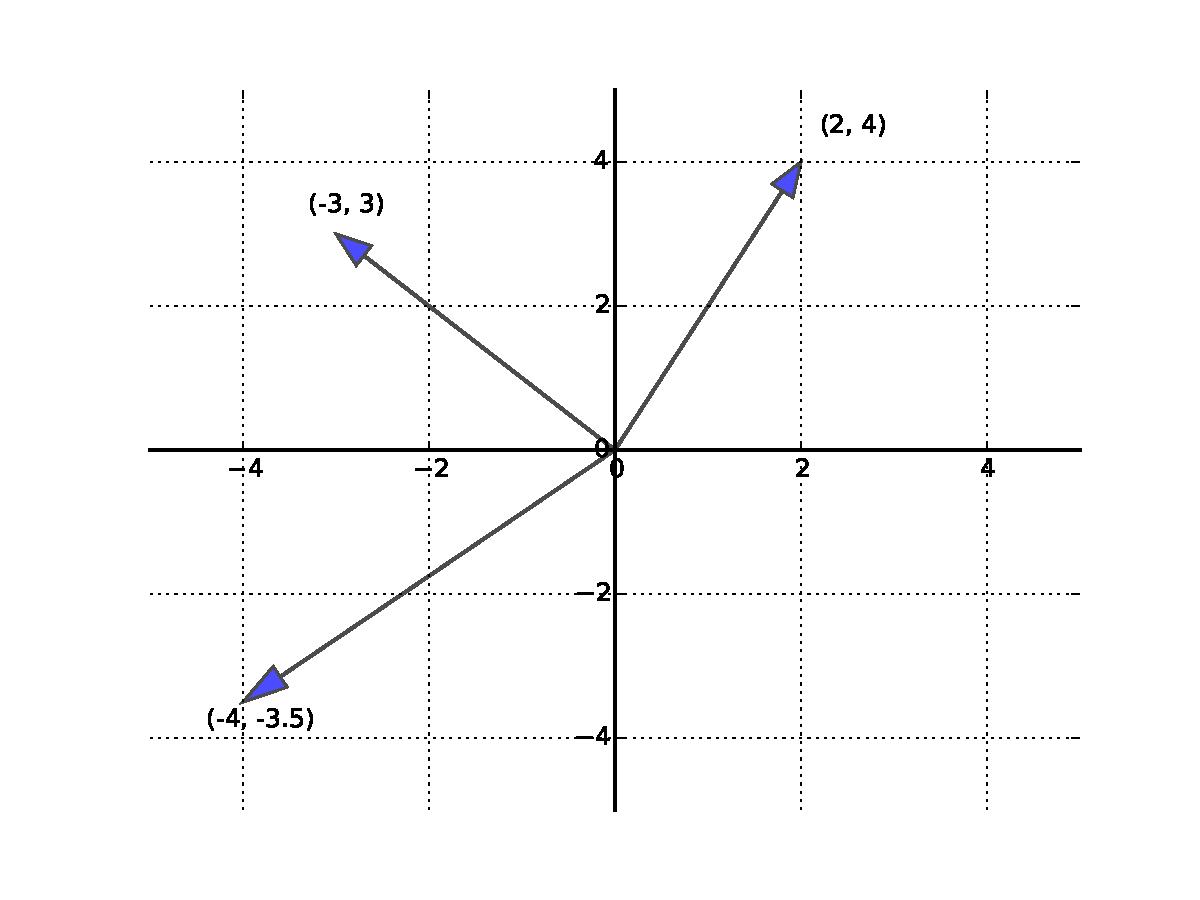
\includegraphics{vecs.pdf}}
        \caption{Три вектора в $\RR^2$ }
       \end{center}
    \end{figure}

\end{frame}


\begin{frame}

    \vspace{2em}
    Вектор из единиц будет обозначен $\boldone$ 
    
    %
    \begin{equation*}
        \boldone := 
        \left(
        \begin{array}{c}
            1 \\
            \vdots \\
            1
        \end{array}
        \right)
    \end{equation*}
    %

    Вектор из нулей будет обозначен $\boldzero$

    %
    \begin{equation*}
        \boldzero := 
        \left(
        \begin{array}{c}
            0 \\
            \vdots \\
            0
        \end{array}
        \right)
    \end{equation*}

\end{frame}


\begin{frame}
    \frametitle{Линейные операции}

    \vspace{2em}
    
    Две базовые алгебраические операции: 
    %
    \begin{enumerate}
        \item Сложение векторов 
        \item Умножение на скаляр
    \end{enumerate}
    
    
    1. \navy{Сумма} $\boldx \in \RR^N$ и $\boldy \in \RR^N$ обозначается
    
    \begin{equation*}
        \boldx + \boldy 
        :=: 
        \left(
        \begin{array}{c}
            x_1 \\
            x_2 \\
            \vdots \\
            x_N
        \end{array}
        \right)
        +
        \left(
        \begin{array}{c}
             y_1 \\
             y_2 \\
            \vdots \\
             y_N
        \end{array}
        \right)
        :=
        \left(
        \begin{array}{c}
            x_1 + y_1 \\
            x_2 + y_2 \\
            \vdots \\
            x_N + y_N
        \end{array}
        \right)
    \end{equation*}
    %


\end{frame}


\begin{frame}

    Пример 1:

    \begin{equation*}
        \left(
        \begin{array}{c}
            1 \\
            2 \\
            3 \\
            4
        \end{array}
        \right)
        +
        \left(
        \begin{array}{c}
             2 \\
             4 \\
             6 \\
             8
        \end{array}
        \right)
        :=
        \left(
        \begin{array}{c}
            3 \\
            6 \\
            9 \\
            12
        \end{array}
        \right)
    \end{equation*}
    %

    Пример 2:

    \begin{equation*}
        \left(
        \begin{array}{c}
            1 \\
            2 \\
            3 \\
            4
        \end{array}
        \right)
        +
        \left(
        \begin{array}{c}
             1 \\
             1 \\
             1 \\
             1
        \end{array}
        \right)
        :=
        \left(
        \begin{array}{c}
            2 \\
            3 \\
            4 \\
            5
        \end{array}
        \right)
    \end{equation*}
    
\end{frame}

\begin{frame}
    

\begin{figure}

  \begin{center}
    \scalebox{.4}{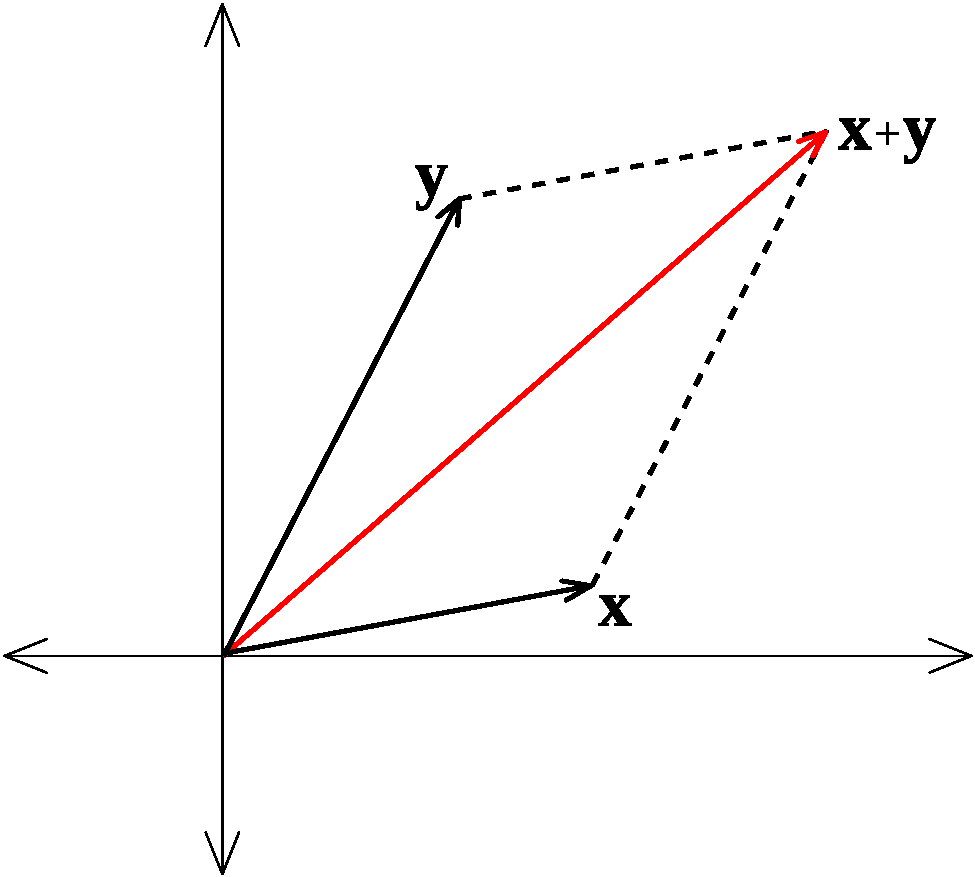
\includegraphics{vec_add.pdf}}
   \caption{\label{f:vec_add} Сложение векторов}
  \end{center}
  
\end{figure}



\end{frame}


\begin{frame}
    
    2. \navy{Умножение на скаляр} $\alpha \in \RR$ и $\boldx \in \RR^N$ обозначается
    
    \begin{equation*}
        \alpha \boldx 
        =
        \alpha \left(
        \begin{array}{c}
            x_1 \\
            x_2 \\
            \vdots \\
            x_N
        \end{array}
        \right)
        :=
        \left(
        \begin{array}{c}
            \alpha x_1 \\
            \alpha x_2 \\
            \vdots \\
            \alpha x_N
        \end{array}
        \right)
    \end{equation*}
    %

\end{frame}



\begin{frame}

    Пример 1:

    \begin{equation*}
        0.5 
        \left(
        \begin{array}{c}
            1 \\
            2 \\
            3 \\
            4
        \end{array}
        \right)
        :=
        \left(
        \begin{array}{c}
            0.5 \\
            1.0 \\
            1.5 \\
            2.0 
        \end{array}
        \right)
    \end{equation*}
    %

    Пример 2:

    \begin{equation*}
        -1
        \left(
        \begin{array}{c}
            1 \\
            2 \\
            3 \\
            4
        \end{array}
        \right)
        :=
        \left(
        \begin{array}{c}
            -1 \\
            -2 \\
            -3 \\
            -4
        \end{array}
        \right)
    \end{equation*}
    %
\end{frame}

\begin{frame}
    
\begin{figure}
  \begin{center}
   \scalebox{.4}{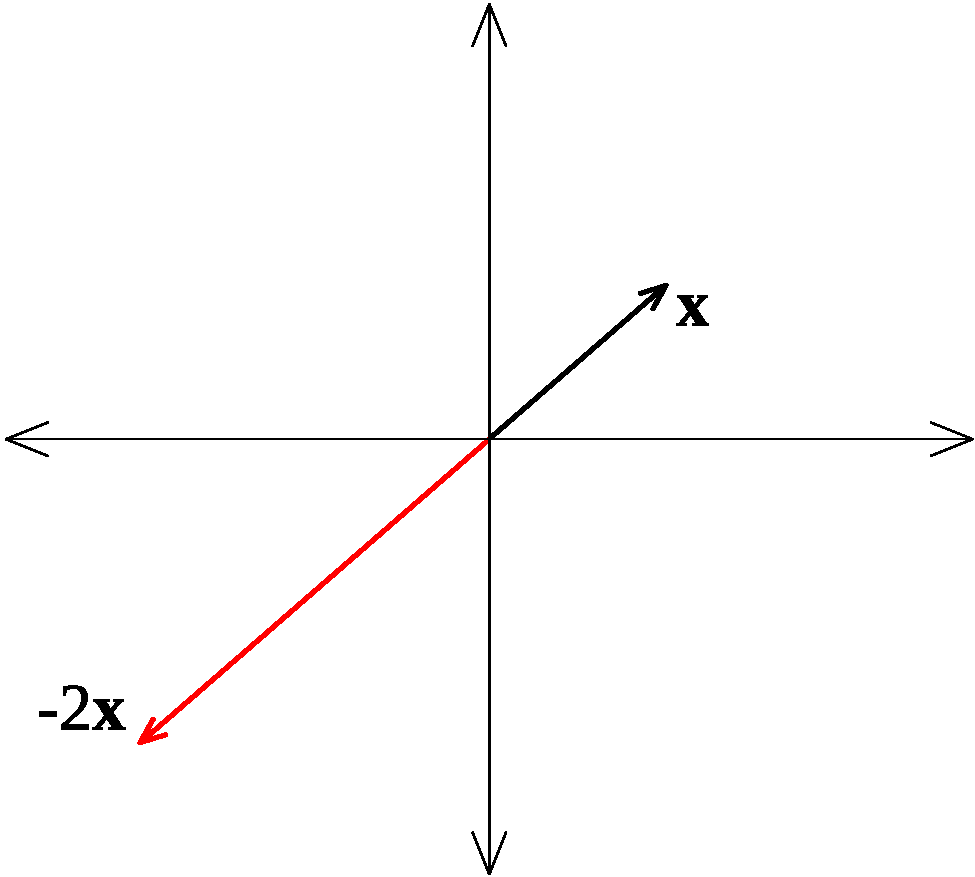
\includegraphics{vec_scalar.pdf}}
    \caption{\label{f:vec_scalar} Уножение на скаляр}
 \end{center}
\end{figure}

\end{frame}



\begin{frame}
    
    \vspace{2em}
    Вычитание выполняется поэлементно, аналогично умножению 

    \begin{equation*}
        \boldx - \boldy 
        :=
        \left(
        \begin{array}{c}
            x_1 - y_1 \\
            x_2 - y_2 \\
            \vdots \\
            x_N - y_N
        \end{array}
        \right)
    \end{equation*}
    
    \vspace{.7em}
    Определение можно дать в терминах сложения и умножения на скаляр

    \begin{equation*}
      \boldx - \boldy := \boldx + (-1) \boldy      
    \end{equation*}

\end{frame}



\begin{frame}

     \vspace{2em}
    \begin{figure}
       \begin{center}
        \scalebox{.375}{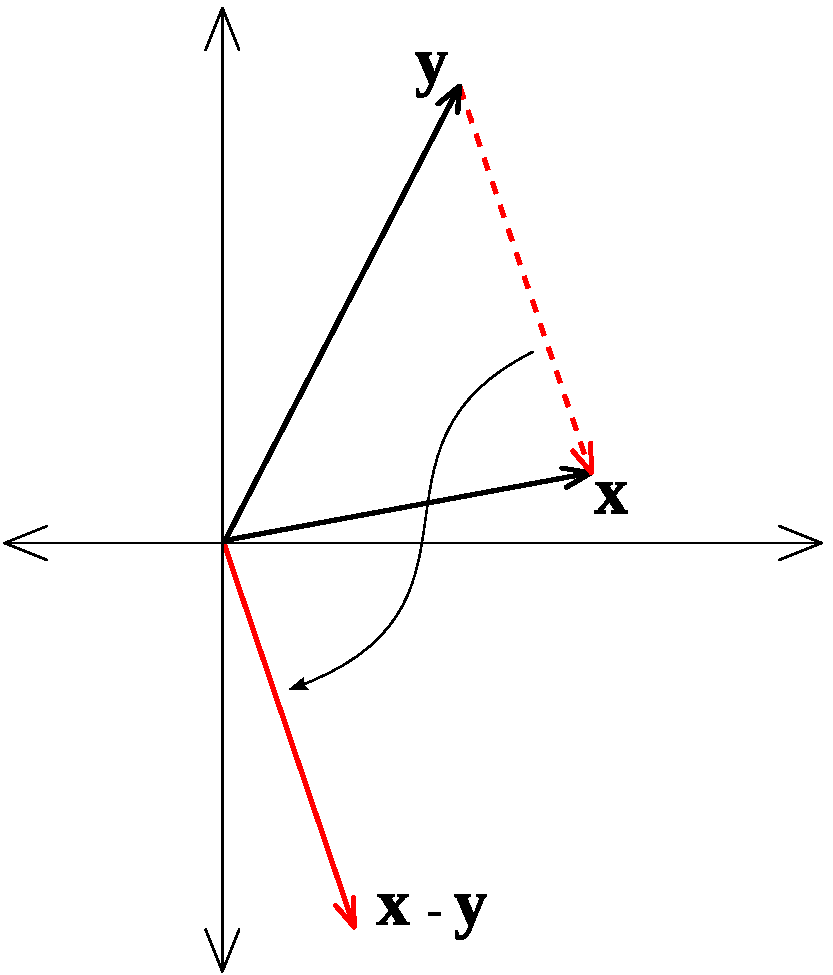
\includegraphics{vec_minus.pdf}}
       \caption{\label{f:vec_minus} Разница векторов}
       \end{center}
    \end{figure}

\end{frame}




%begin{frame}[fragile]
    
%    Incidentally, most high level numerical libraries treat vector addition
%    и scalar multiplication in the same way --- elementwise

%\begin{pythoncode}
%    In [1]: import numpy as np

%    In [2]: x = np.array((2, 4, 6))

%    In [3]: y = np.array((10, 10, 10))

%    In [4]: x + y  # Vector addition
%    Out[4]: array([12, 14, 16])

%    In [6]: 2 * x  # Scalar multiplication
%    Out[6]: array([ 4,  8, 12])
%\end{pythoncode}


%\end{frame}

\begin{frame}
    \frametitle{Скалярное произведение}
    
     \vspace{2em}
    \navy{Скалярное произведение} двух векторов $\boldx$ и $\boldy$ в $\RR^N$ обозначается $\inner{\boldx,  \boldy}$, и является суммой произведения их элементов:
    
    \vspace{.7em}
    \begin{equation*}
        \label{eq:dipv}
        \inner{\boldx,  \boldy} := \sum_{n=1}^N x_n y_n 
    \end{equation*}
    
    
\end{frame}


%\begin{frame}[fragile]


%    \begin{pythoncode}
%In [1]: import numpy as np

%In [2]: x = np.array((1, 2, 3, 4))

%In [3]: y = np.array((2, 4, 6, 8))

%In [6]: np.sum(x * y)  # Inner product
%Out[6]: 60
%    \end{pythoncode}
    
%\end{frame}

\begin{frame}

    \vspace{2em}
    \Fact \eqref{ET-fa:profno}
    
    Для любых $\alpha, \beta \in \RR$ и любых $\boldx, \boldy \in \RR^N$, верны следующие утверждения:
    %
    \begin{enumerate}
        \item $\inner{\boldx, \boldy} = \inner{\boldy, \boldx}$,
        \item $\inner{\alpha \boldx, \beta \boldy} =  \alpha \beta
            \inner{\boldx, \boldy}$, и
        \item $\inner{\boldx, \alpha \boldy + \beta \boldz} =  \alpha
            \inner{\boldx, \boldy} + \beta \inner{\boldx, \boldz}$.
    \end{enumerate}
    
    \vspace{1em}
    Свойства можно легко проверить с помощью определений умножения на скаляр и скалярного произведения.

    Для 2., например, возьмите любые $\alpha, \beta \in \RR$ и любые $\boldx, \boldy \in
    \RR^N$:
    %
    \begin{equation*}
        \inner{\alpha \boldx, \beta \boldy}
        = \sum_{n=1}^N \alpha x_n \beta y_n
        = \alpha \beta \sum_{n=1}^N x_n y_n 
        = \alpha \beta \inner{\boldx, \boldy}
    \end{equation*}

\end{frame}

\begin{frame}
    \frametitle{Нормы и расстояние}
    
     \vspace{2em}
    \navy{Норма} (Эвклида) $\boldx \in \RR^N$ обозначается
    %
    \begin{equation*}
        \label{eq:eucnorm}
        \| \boldx \| := \sqrt{\inner{\boldx, \boldx}} 
    \end{equation*}
    %
    
    \vspace{.7em}
    Интерпретация:
    %
    \begin{itemize}
        \item $\| \boldx \|$ показывает ``длину'' вектора $\boldx$
            \vspace{0.5em}
        \item $\| \boldx - \boldy \|$ показывает расстояние между векторами $\boldx$ и $\boldy$
    \end{itemize}

\end{frame}

%\begin{frame}
    
%    \begin{figure}
%       \begin{center}
%           \scalebox{.95}{\input{../figs_code/tikzfigs/vec.tex}}
%        \caption{\label{f:vec_rpt} Length of red line $= \sqrt{x_1^2 + x_2^2}
%            =: \|\boldx\|$ }
%       \end{center}
%    \end{figure}

%\end{frame}

\begin{frame}
    
    \vspace{2em}
    \Fact\eqref{ET-fa:profno} Для любого $\alpha \in \RR$ и любых $\boldx, \boldy \in \RR^N$, верны следующие утверждения:
    \begin{enumerate}
        \item $\| \boldx \| \geq 0$ и $\| \boldx \| = 0$ тогда и только тогда, когда
            $\boldx = \boldzero$
            \vspace{1em}
        \item $\| \alpha \boldx \| = |\alpha| \| \boldx \|$
            \vspace{1em}
        \item $\| \boldx + \boldy \| \leq  \| \boldx \| + \| \boldy \|$
            (\navy{неравенство треугольника})
            \vspace{1em}
        \item $|\inner{\boldx, \boldy}| \leq  \| \boldx \| \| \boldy \|$
            (\navy{неравенство Коши — Буняковского})
    \end{enumerate}

\end{frame}

\begin{frame}

    \vspace{2em}
    Свойства 1. и 2. легко доказать (упражнение)
    
    Свойство 4. рассматривается в ET упражнении \ref{ET-ex:pcsin}
    
    \vspace{.7em}
    Покажем доказательство свойства 3. с помощью свойств скалярного произведения (факт \ref{ET-fa:innpp})
    
    \begin{align*}
        \label{eq:tifcs}
         \| \boldx + \boldy \|^2
        & = \inner{\boldx + \boldy, \boldx + \boldy}
        \\& = \inner{\boldx, \boldx} + 2 \inner{\boldx, \boldy} +  \inner{\boldy,
        \boldy}
        \\& \leq \inner{\boldx, \boldx} + 2 | \! \inner{\boldx, \boldy} \! | +  \inner{\boldy,
        \boldy}
    \end{align*}
    %
\end{frame}

\begin{frame}
    
     \vspace{2em}
    Применим неравенство Коши — Буняковского
    
    \begin{equation*}
        \| \boldx + \boldy \|^2 \leq ( \| \boldx \| + \| \boldy\|)^2
    \end{equation*}
    
      \vspace{.7em}
    Убираем квадраты и получаем неравенство треугольника
    
\end{frame}


\begin{frame}
    
    \vspace{2em}
    \navy{Линейная комбинация} векторов $\boldx_1,\ldots, \boldx_K$ in $\RR^N$ 
    --- это вектор 
    %
    \begin{equation*}
        \boldy = \sum_{k=1}^K \alpha_k \boldx_k 
        =  \alpha_1 \boldx_1 + \cdots +  \alpha_K \boldx_K 
    \end{equation*}
    %
    где $\alpha_1,\ldots, \alpha_K$ скаляры

    \vspace{.7em}

    \Eg
    
    \begin{equation*}
        0.5 \left(
        \begin{array}{c}
            6.0 \\
            2.0 \\
            8.0
        \end{array}
        \right)
        +
        3.0 \left(
        \begin{array}{c}
             0 \\
             1.0 \\
             -1.0
        \end{array}
        \right)
        =
        \left(
        \begin{array}{c}
            3.0 \\
            4.0 \\
            1.0
        \end{array}
        \right)
    \end{equation*}
    %

\end{frame}

\begin{frame}
    

    \begin{figure}
       \begin{center}
           \scalebox{.375}{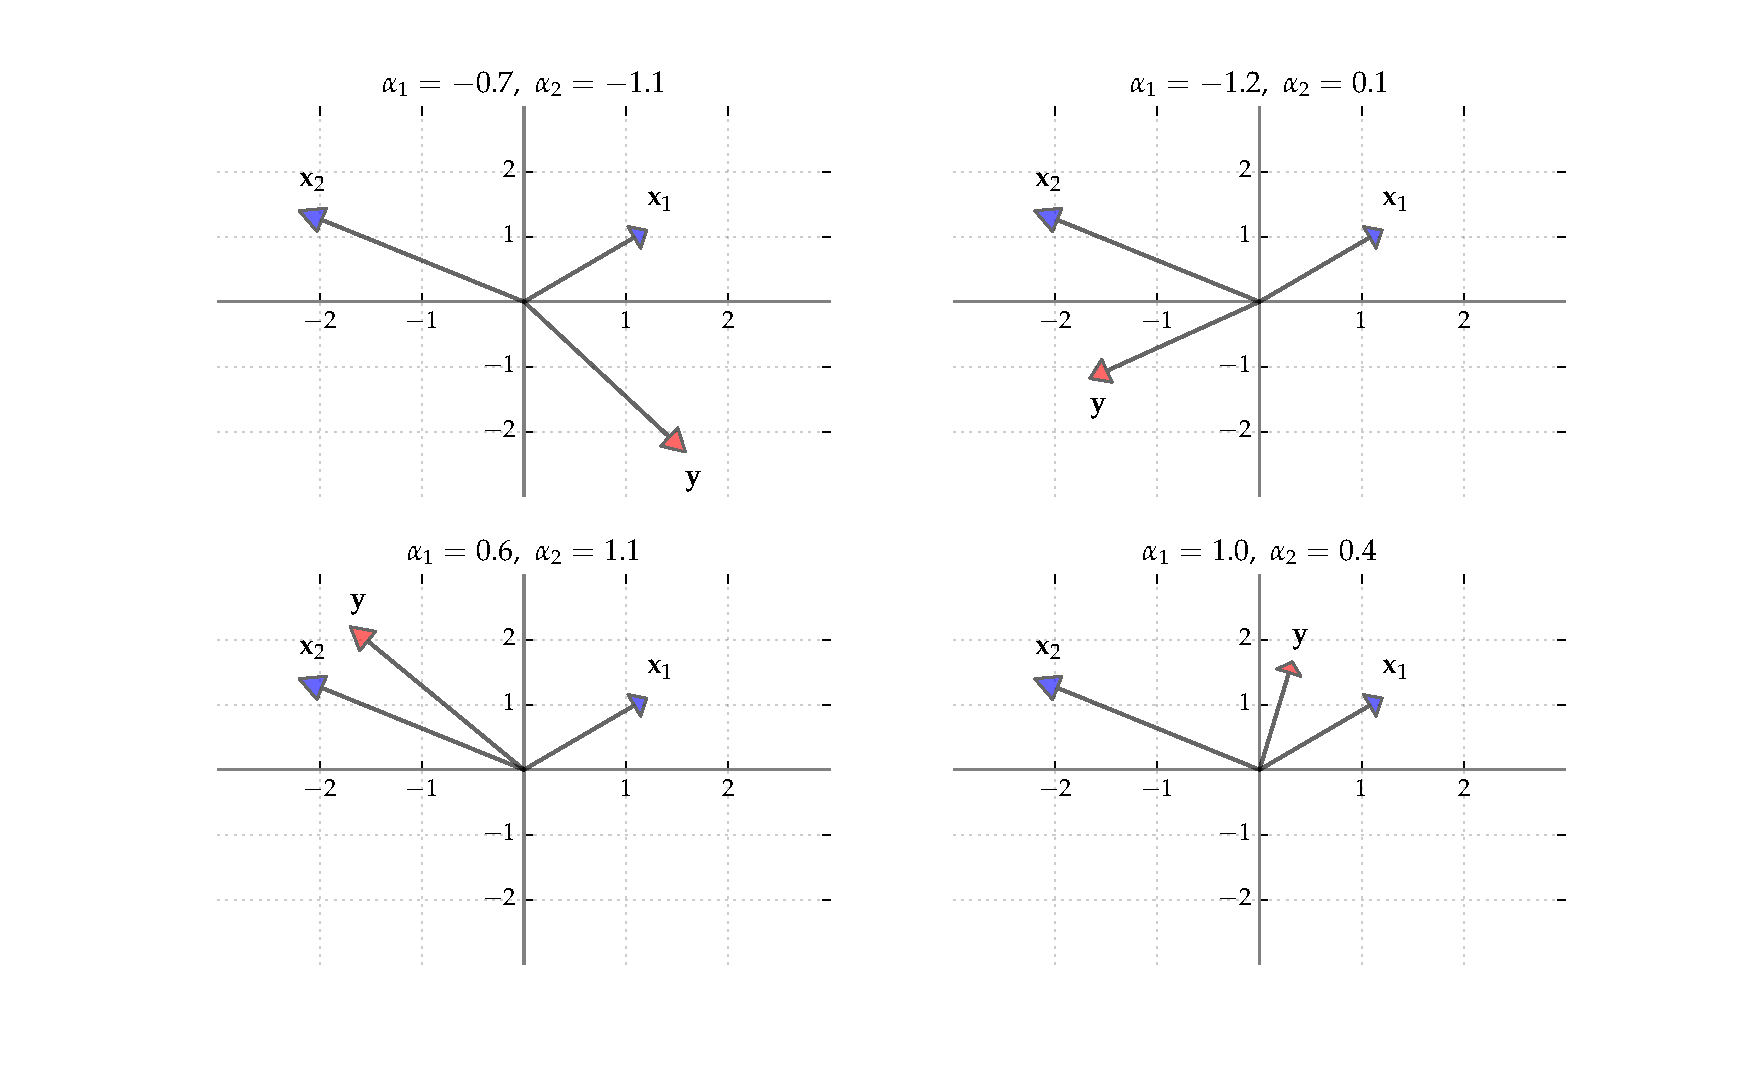
\includegraphics[trim={4em 4em 4em 1em}, clip]{lin_comb.pdf}}
        \caption{\label{f:lin_comb} Линейные комбинации $\boldx_1, \boldx_2$}
       \end{center}
    \end{figure}

\end{frame}

\begin{frame}

    \frametitle{Линейная оболочка}

    \vspace{2em}
    Пусть $X \subset \RR^N$ некое непустое множество

    \vspace{1em}

    Множество всех возможных линейных комбинаций $X$ называют \navy{линейной оболочкой} $X$, обозначается $\Span(X)$

    \vspace{.7em}

    Для конечного $X := \{\boldx_1,\ldots, \boldx_K\}$ линейную оболочку можно записать так 
    
    \begin{equation*}
        \Span(X):= \left\{ \text{ все } \sum_{k=1}^K \alpha_k \boldx_k 
        \text{, где }
         (\alpha_1,\ldots, \alpha_K) \in \RR^K \right\}
    \end{equation*}
    
\end{frame}

\begin{frame}

    \vspace{2em}
    \Eg
    Четыре вектора, обозначенные $\boldy$ 
    на предыдущем рисунке, лежат в линейной оболочке $X = \{\boldx_1, \boldx_2\}$
    
    \vspace{.7em}
    Может ли \emph{любой} вектор в $\RR^2$ быть создан линейной комбинацией $\boldx_1, \boldx_2$?  
    
    Ответ да. Мы докажем это в \S\ref{ET-ss:bad}
    
\end{frame}



\begin{frame}
    
    \vspace{2em}
    \Eg
    Пусть $X = \{ \boldone \} \subset \RR^2$, где $\boldone := (1,1)$  
    
    Линейная оболочка $X$ состоит из всех векторов вида 
    %
    \[
    \alpha \boldone 
    =
    \left(
    \begin{array}{c}
        \alpha \\
        \alpha
    \end{array}
    \right)
    \quad \text{, где } \quad \alpha \in \RR  
    \]
   
    \vspace{2em}
    Представляет собой прямую на плоскости, которая проходит через
    %
    \begin{itemize}
        \item вектор $\boldone$  (при $\alpha = 1$)
        \item начало координат $\boldzero$ (при $\alpha = 0$)
    \end{itemize}

\end{frame}

\begin{frame}

    \vspace{2em}
    \begin{figure}
       \centering
        \scalebox{.4}{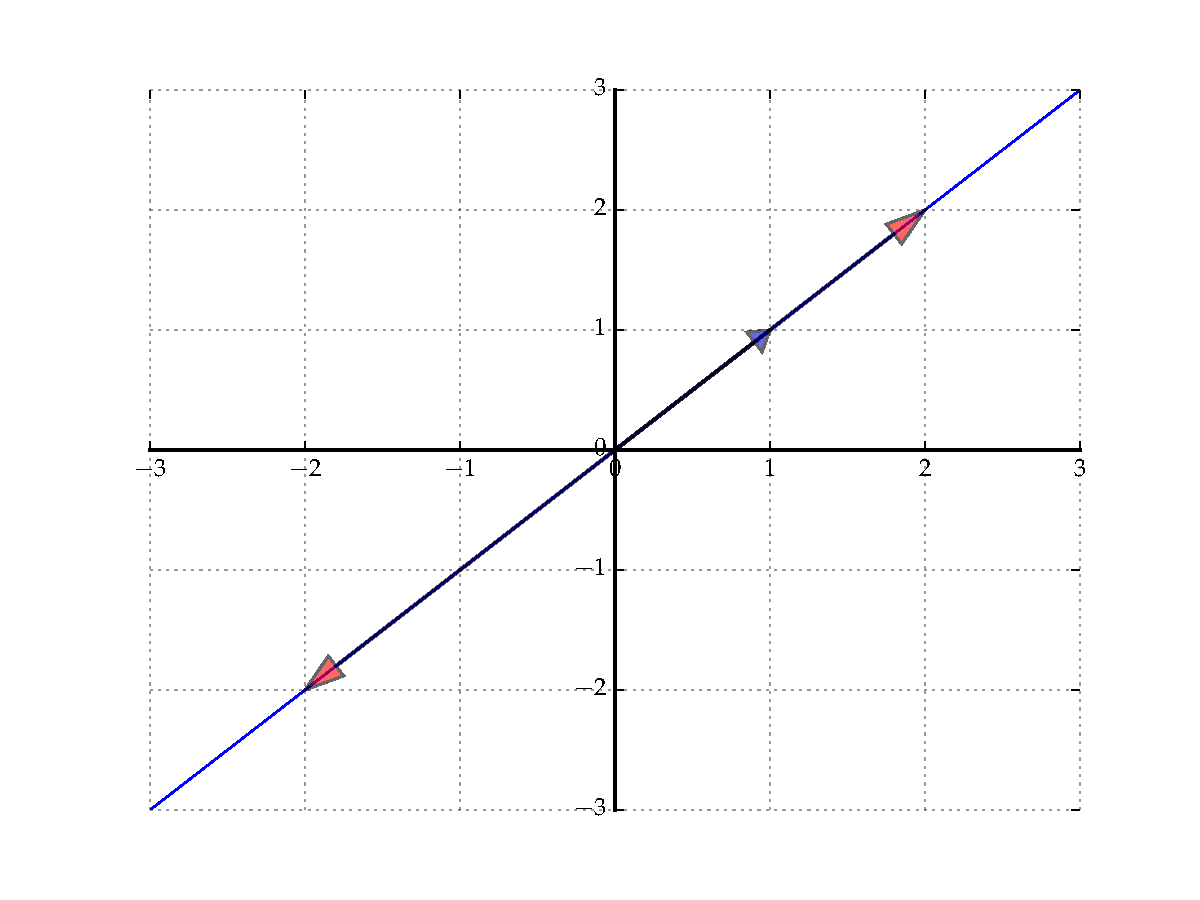
\includegraphics{span_of_one_vec.pdf}}
        \caption{Линейная оболочка $\boldone := (1,1)$ в $\RR^2$}
    \end{figure}

\end{frame}

\begin{frame}
    
    \vspace{2em}
    \Eg
    Набор канонически базисных векторов $\{\bolde_1, \ldots, \bolde_N\}$
    линейно независим в $\RR^N$
    
    \Prf Пусть $\alpha_1, \ldots, \alpha_N$ коэффициенты, такие что
    $\sum_{k=1}^N \alpha_k \bolde_k = \boldzero$

    Эквивалентно,
    %
    \begin{equation*}
        \left(
        \begin{array}{c}
            \alpha_1 \\
            \alpha_2 \\
            \vdots \\
            \alpha_N
        \end{array}
        \right)
        = \sum_{k=1}^N \alpha_k \bolde_k 
        = \boldzero
        =
        \left(
        \begin{array}{c}
            0 \\
            0 \\
            \vdots \\
            0
        \end{array}
        \right)
    \end{equation*}

    \vspace{1em}

    В частности, $\alpha_k = 0$ для всех $k$
    
\end{frame}




\begin{frame}

    \vspace{2em}
    \Eg
    Пусть $\boldx_1 = (3, 4, 2)$ и $\boldx_2 = (3, -4, 0.4)$

    \vspace{1em}
    По определению, линейная оболочка --- все возможные вектора в виде

    \begin{equation*}
        \boldy = 
        \alpha \left(
        \begin{array}{c}
            3 \\
            4 \\
            2
        \end{array}
        \right)
        +
        \beta \left(
        \begin{array}{c}
             3 \\
             -4 \\
             0.4
        \end{array}
        \right)
        \quad \text{, где} \quad
        \alpha, \beta \in \RR
    \end{equation*}
    %
    
    Это плоскость, проходящая через
    %
    \begin{itemize}
        \item вектор $\boldx_1$
        \item вектор $\boldx_2$
        \item начало координат $\boldzero$
    \end{itemize}


\end{frame}


\begin{frame}

    \vspace{2em}
   \begin{figure}
       \scalebox{.40}{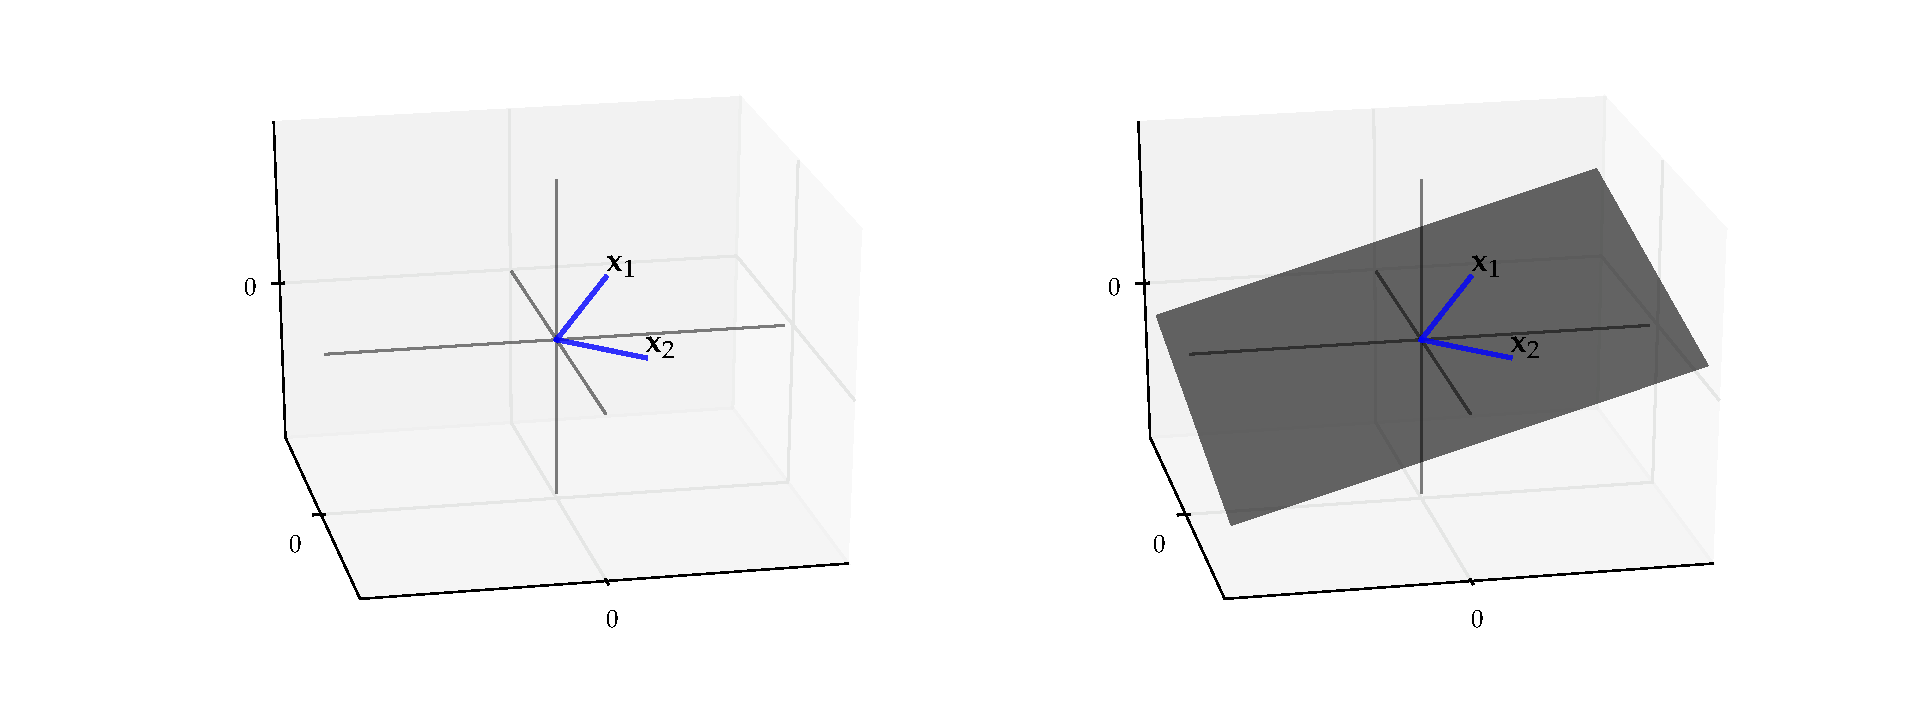
\includegraphics[trim=110 0 50 10, clip]{span_plane.pdf}}
       \caption{\label{f:span_plane} Линейная оболочка $\boldx_1, \boldx_2$}
   \end{figure}

\end{frame}




%\begin{frame}
    
%    Let $Y$ be any subset of $\RR^N$, и let $X:= \{\boldx_1,\ldots, \boldx_K\}$ 
%    
%    \vspace{1em}
%
%   If $Y \subset \Span(X)$, we say that the vectors in $X$ \navy{span the set} $Y$
    
%    \vspace{1em}

 %   Alternatively, we say that $X$ is a \navy{spanning set} for $Y$

%    \vspace{1em}
    
%    A nice situation: $Y$ is large but $X$ is small
    
%    \vspace{1em}
%    $\implies$ large set $Y$ ``described'' by the small number of vectors in $X$
%\end{frame}


\begin{frame}
    
    \vspace{2em}
    \Eg 
    Рассмотрим векторы $\{\bolde_1, \ldots, \bolde_N\} \subset \RR^N$, где

    \begin{equation*}
        \bolde_1 := 
        \left(
        \begin{array}{c}
            1 \\
            0 \\
            \vdots \\
            0
        \end{array}
        \right),
        \quad 
        \bolde_2 := 
        \left(
        \begin{array}{c}
            0 \\
            1 \\
            \vdots \\
            0
        \end{array}
        \right),
        \; 
        \cdots,
        \;
        \bolde_N := 
        \left(
        \begin{array}{c}
            0 \\
            0 \\
            \vdots \\
            1
        \end{array}
        \right)
    \end{equation*}
    %

    \vspace{1em}

    $\bolde_n$ состоит из нулей, кроме $n$-ого элемента равного $1$
    
    \vspace{1em}

    Вектора $\bolde_1, \ldots, \bolde_N$ назвают
    \navy{каноническими базисными векторами} of $\RR^N$

\end{frame}

\begin{frame}

    \begin{figure}
       \begin{center}
        \begin{tikzpicture}[
    scale=5,
    axis/.style={<->, >=stealth'},
    important line/.style={thick},
    dashed line/.style={dashed, thin},
    every node/.style={color=black}
    ]

    % define x,y
    \coordinate(O) at (0,0);
    \coordinate (X) at (0.7,0.4);
    \coordinate (e1) at (0.5,0);
    \coordinate (e2) at (0,0.5);
    % axis
    \draw[axis] (-0.3,0)  -- (0.9,0) node(xline)[right] {};
    \draw[axis] (0,-0.2) -- (0,0.7) node(yline)[above] {};
    % x, y, x+y
    \draw[important line, ->]  (O) -- (e1) node[above, text width=5em] {$\bolde_1 = (1,0)$};
    \draw[important line, ->]  (O) -- (e2) node[right, text width=5em] {$\bolde_2 = (0,1)$};
    \draw[important line, red, ->]  (O) -- (X) node[right] {$\boldy = y_1 \bolde_1 + y_2 \bolde_2$};
\end{tikzpicture}

        \caption{\label{f:vec_canon} Базисные векторы в $\RR^2$}
       \end{center}
    \end{figure}

\end{frame}


\begin{frame}
    
    \vspace{2em}
    \Eg (прод.) 
    
    Линейная оболочка $\{\bolde_1, \ldots, \bolde_N\}$ эквивалентна всему $\RR^N$
    
    Доказательство для $N=2$: 
    
    Пусть $\boldy \in \RR^2$, тогда
    %
    \begin{align*}
        \boldy 
        :=
        \left(
        \begin{array}{c}
            y_1 \\
            y_2
        \end{array}
        \right)
        & =
        \left(
        \begin{array}{c}
            y_1 \\
            0
        \end{array}
        \right)
        +
        \left(
        \begin{array}{c}
            0 \\
            y_2
        \end{array}
        \right)
        \\
        & =
        y_1
        \left(
        \begin{array}{c}
            1 \\
            0
        \end{array}
        \right)
        +
        y_2
        \left(
        \begin{array}{c}
            0 \\
            1
        \end{array}
        \right)
        = y_1 \bolde_1 + y_2 \bolde_2
    \end{align*}
    %
    Таким образом, $\boldy \in \Span \{\bolde_1, \bolde_2\}$ 
    
    Так как $\boldy$ произвольный, мы показали, что $\Span \{\bolde_1,
    \bolde_2\} = \RR^2$

\end{frame}

%\begin{frame}
    
    %\begin{figure}
    %   \begin{center}
     %   \scalebox{.95}{\begin{tikzpicture}[
    scale=5,
    axis/.style={<->, >=stealth'},
    important line/.style={thick},
    dashed line/.style={dashed, thin},
    every node/.style={color=black}
    ]

    % define x,y
    \coordinate(O) at (0,0);
    \coordinate (X) at (0.7,0.4);
    \coordinate (e1) at (0.5,0);
    \coordinate (e2) at (0,0.5);
    % axis
    \draw[axis] (-0.3,0)  -- (0.9,0) node(xline)[right] {};
    \draw[axis] (0,-0.2) -- (0,0.7) node(yline)[above] {};
    % x, y, x+y
    \draw[important line, ->]  (O) -- (e1) node[above, text width=5em] {$\bolde_1 = (1,0)$};
    \draw[important line, ->]  (O) -- (e2) node[right, text width=5em] {$\bolde_2 = (0,1)$};
    \draw[important line, red, ->]  (O) -- (X) node[right] {$\boldy = y_1 \bolde_1 + y_2 \bolde_2$};
\end{tikzpicture}
}
     %   \caption{\label{f:vec_canon2} Canonical basis vectors in $\RR^2$}
    %   \end{center}
   % \end{figure}

%\end{frame}


\begin{frame}
    
    \vspace{2em}
    \Eg 
    Рассмотрим множество 
    %
    \begin{equation*}
        P := \setntn{(x_1, x_2, 0) \in \RR^3}{ x_1, x_2 \in \RR}
    \end{equation*}
    %
    Графически, $P =$ плоскость в $\RR^3$с координатой высоты $=0$
    %
    \begin{figure}
       \begin{center}
        \scalebox{.35}{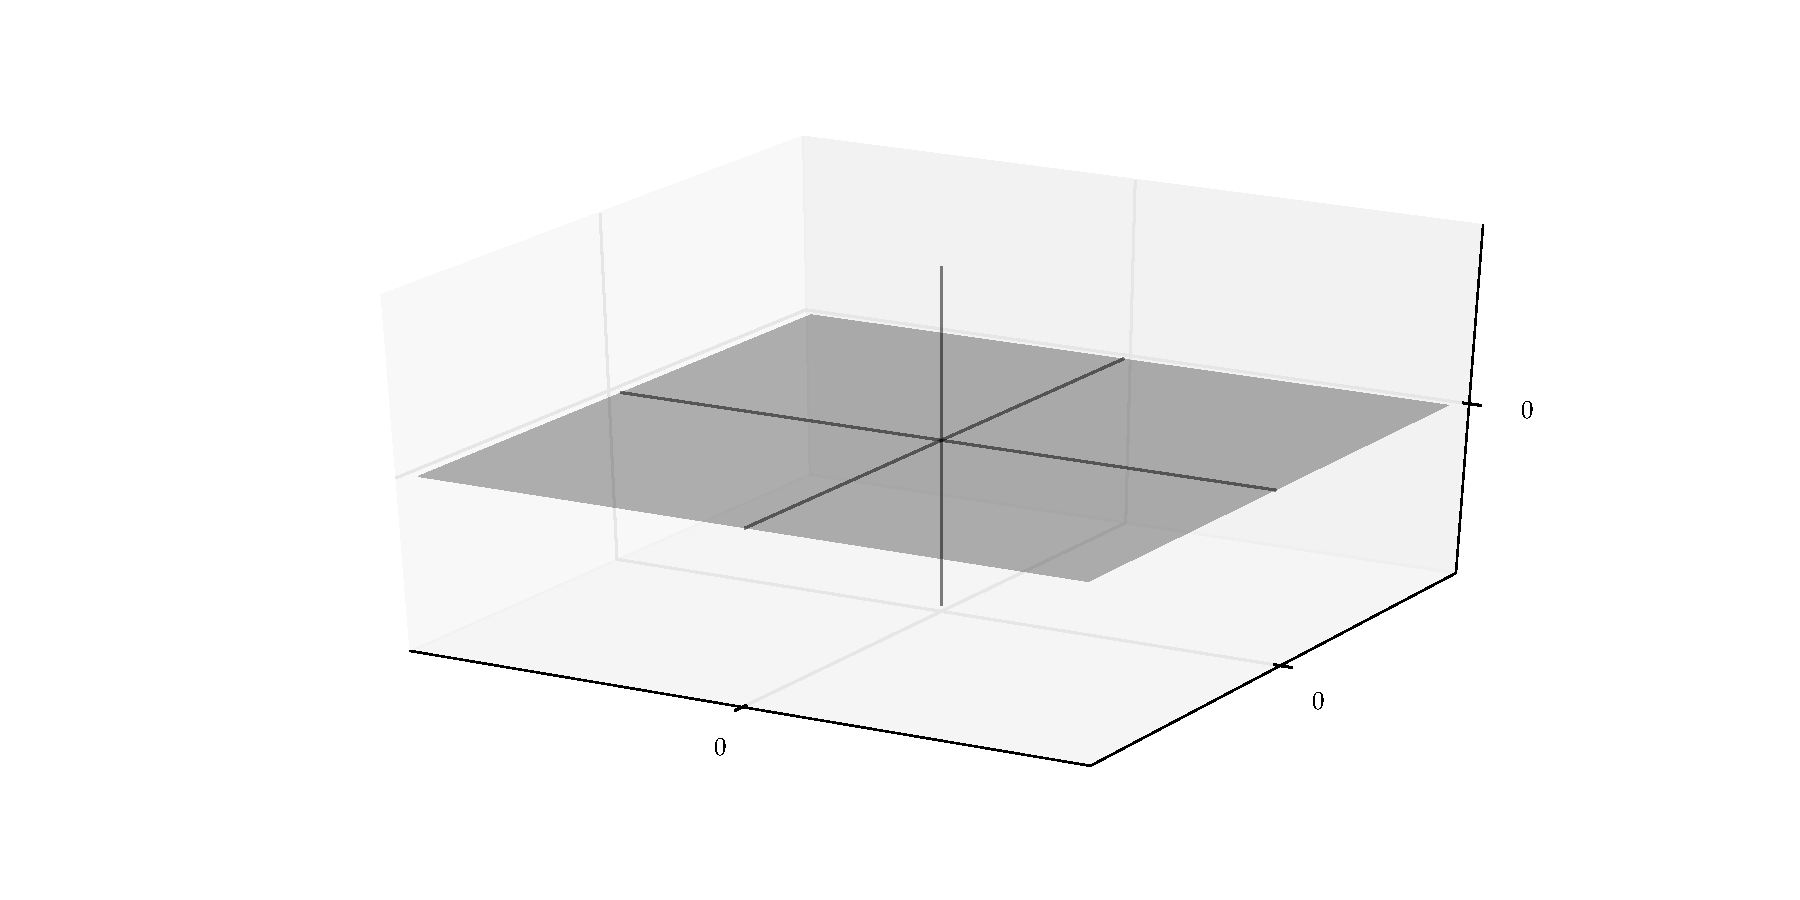
\includegraphics[trim={4em 6em 4em 1em}, clip]{flat_plane_no_vecs.pdf}}
       \end{center}
    \end{figure}

\end{frame}



\begin{frame}

    \vspace{2em}
    \Eg (прод.)
    
    Если $\bolde_1 = (1,0,0)$ и $\bolde_2=(0,1,0)$, тогда $\Span\{\bolde_1, \bolde_2\} = P$ 
    
   Чтобы подтвердить утверждение, возьмем $\boldx = (x_1, x_2, 0)$, любой элемент $P$. 
   Можно записать $\boldx$ в следующем виде  
    %
    \begin{equation*}
        \boldx = 
        \left(
        \begin{array}{c}
            x_1 \\
            x_2 \\
            0
        \end{array}
        \right)
        =
        x_1
        \left(
        \begin{array}{c}
            1 \\
            0 \\
            0
        \end{array}
        \right)
        + 
        x_2
        \left(
        \begin{array}{c}
            0 \\
            1 \\
            0
        \end{array}
        \right)
        = x_1 \bolde_1 + x_2 \bolde_2
    \end{equation*}
    %

    Другими словами, $P \subset \Span\{\bolde_1, \bolde_2\}$

    И наоборот, у нас имеется $\Span\{\bolde_1, \bolde_2\} \subset P$ (почему?)


\end{frame}


\begin{frame}

    \vspace{2em}
    \begin{figure}
       \begin{center}
        \scalebox{.4}{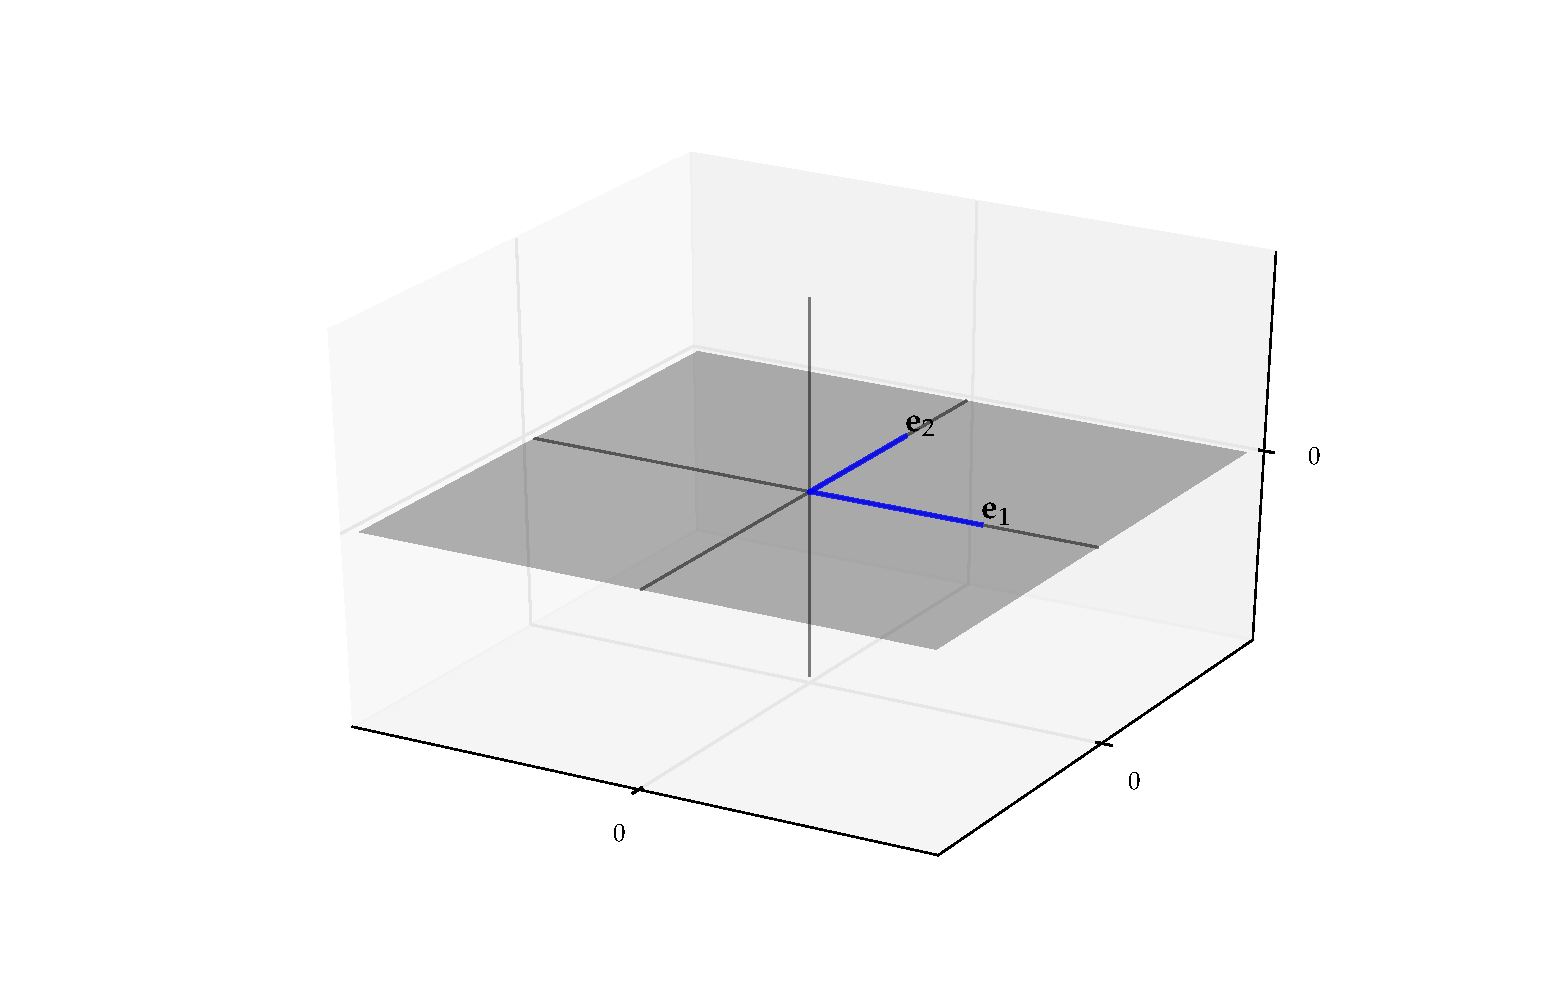
\includegraphics[trim={4em 4em 4em 1em}, clip]{flat_plane_e_vecs.pdf}}
       \end{center}
       \caption{$\Span\{\bolde_1, \bolde_2\} = P$}
    \end{figure}


\end{frame}

\begin{frame}
    
    \vspace{2em}
    \Fact{\eqref{ET-fa:xsys}} 
    Если $X$ и $Y$ непустые подмножества $\mathbb{R}^{N}$ и $X \subset Y$, 
    тода $\Span(X) \subset \Span(Y)$
    \vspace{2em}
    
    \Prf
    Возьмем любой непустой $X \subset Y \subset \RR^N$
    
    Пусть $\boldz \in \Span(X)$, тогда имеется
    %
    \begin{equation*}
        \boldz = \sum_{k=1}^K \alpha_k \boldx_k 
        \text{ для некоторых }
        \boldx_1, \ldots, \boldx_K \in X, \; 
        \alpha_1, \ldots, \alpha_K \in \RR
    \end{equation*}
    
\end{frame}

\begin{frame}

   \vspace{2em}
    \Prf(прод.)
    Так как $X \subset Y$, каждый $\boldx_k$ также находится в $Y$, получается
    %
    \begin{equation*}
        \boldz = \sum_{k=1}^K \alpha_k \boldx_k 
        \text{ для некоторых }
        \boldx_1, \ldots, \boldx_K \in Y, \; 
        \alpha_1, \ldots, \alpha_K \in \RR
    \end{equation*}

    \vspace{.7em}
    Значит, $\boldz \in \Span(Y)$

\end{frame}


\begin{frame}
    \frametitle{Линейная независимость}
    
    \vspace{2em}
    Важные вопросы:

    \begin{itemize}
        \item Когда матрица обратима?
        \item Когда аргументы регрессии страдают от коллинеарности?
        \item Когда система линейных уравнений имеет решение?
    \end{itemize}

    Все эти вопросы тесно связаны с линейной независимостью 

\end{frame}


\begin{frame}

    \vspace{2em}
   

    Непустое множество векторов $X := \{\boldx_1,\ldots, \boldx_K\}
    \subset \RR^N$ называется \navy{линейно независимым}, если
    %
    \begin{equation*}
        \sum_{k=1}^K \alpha_k \boldx_k
         = \boldzero 
        \; \implies \;
        \alpha_1 = \cdots = \alpha_K = 0
    \end{equation*}

    \vspace{1em}

\end{frame}


\begin{frame}
    
    \vspace{2em}
    \Eg 
    Рассмотрим $\boldx_1 = (1.2, 1.1)$ и $\boldx_2 = (-2.2, 1.4)$
    
    Пусть $\alpha_1$ и $\alpha_2$ скаляры, такие что
    %
    \begin{equation*}
        \alpha_1
        \left(
        \begin{array}{c}
            1.2 \\
            1.1
        \end{array}
        \right)
        + 
        \alpha_2
        \left(
        \begin{array}{c}
            -2.2 \\
            1.4
        \end{array}
        \right)
        =
        \boldzero
    \end{equation*}
    
    Это является линейной системой из двух уравнений $\alpha_1$ и $\alpha_2$ 
    
    Единственное решение $\alpha_1 = \alpha_2 = 0$
    
    $\{\boldx_1, \boldx_2\}$ линейно независимы


\end{frame}

    \begin{frame}
        \begin{figure}
       \begin{center}
           \scalebox{.46}{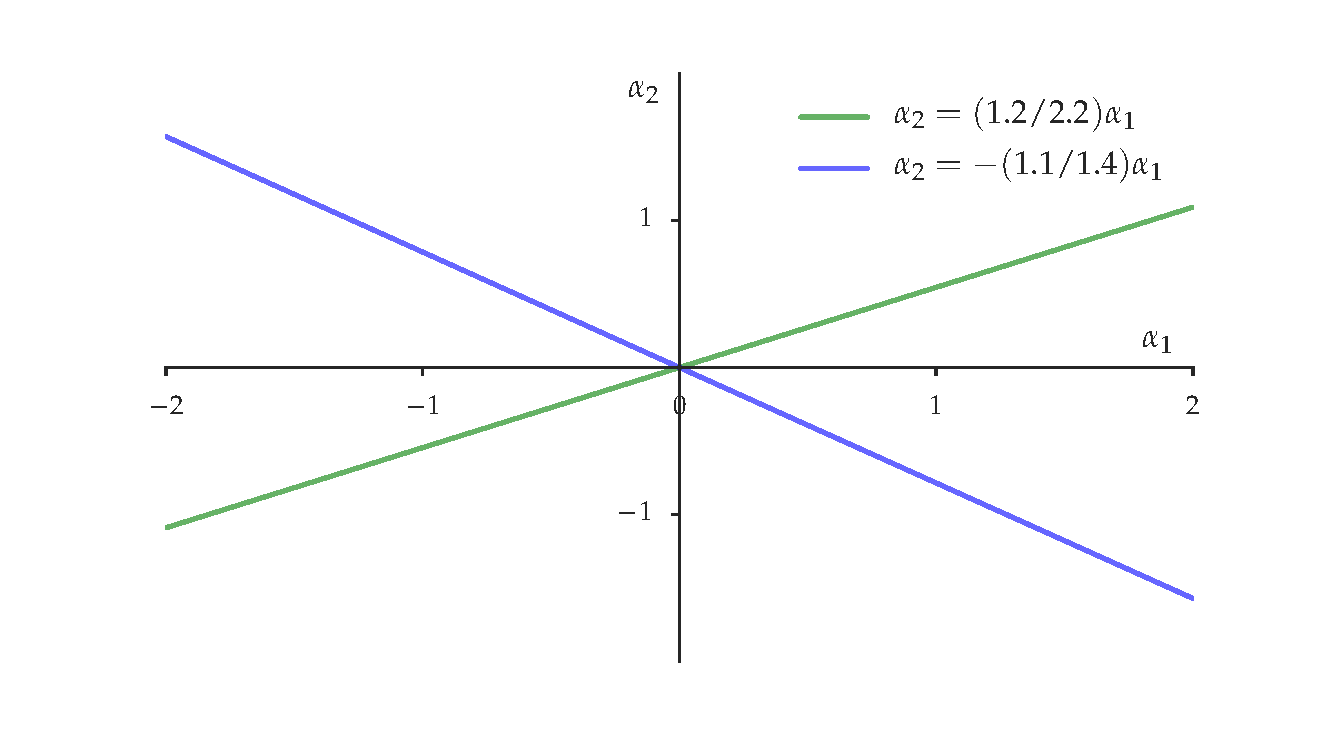
\includegraphics[trim={0 4em 0 1em}, clip]{alpha_eq.pdf}}
           \caption{\label{f:alpha_eq} Единственное решение $\alpha_1 = \alpha_2 = 0$}
       \end{center}
    \end{figure}

\end{frame}

\begin{frame}
    
    \vspace{2em}
    \Eg Базисные векторы $\{\bolde_1, \ldots, \bolde_N\}$
    линейно независимы в $\RR^N$

    Проверим это. Пусть $\alpha_1, \ldots, \alpha_N$ коэффициенты, такие что
    $\sum_{k=1}^N \alpha_k \bolde_k = \boldzero$, тогда
    %
    \begin{equation*}
        \left(
        \begin{array}{c}
            \alpha_1 \\
            \alpha_2 \\
            \vdots \\
            \alpha_N
        \end{array}
        \right)
        = \sum_{k=1}^N \alpha_k \bolde_k 
        = \boldzero
        =
        \left(
        \begin{array}{c}
            0 \\
            0 \\
            \vdots \\
            0
        \end{array}
        \right)
    \end{equation*}

    То есть $\alpha_k = 0$ для всех $k$
    
    Таким образом, $\{\bolde_1, \ldots, \bolde_N\}$ линейно независимы

\end{frame}

\begin{frame}

    \vspace{2em}
    \Thm\eqref{ET-t:fdlinin}
        Пусть $X := \{\boldx_1,\ldots, \boldx_K\} \subset \RR^N$.  Для $K > 1$, следующие утверждения эквивалентны:
        %
        \begin{enumerate}
            \item $X$ линейно независим
            \item $X_0$ --- подходящее подмножество $X$
                $\,\implies\,$ $\Span X_0$ --- подходящее подмножество $\Span X$
            \item Ни один из векторов $X$ не может быть записан как линейная комбинация оставшихся
        \end{enumerate}
        %
    Доказательство есть в упражнениях. См. ET упр. \ref{ET-ex:ott} и решение
    
\end{frame}

\begin{frame}

    \vspace{2em}
    \Eg 
    Если убрать любой базисный вектор, линейная оболочка уменьшится

    Рассмотрим случай с $N=2$
    
    Мы знаем, что $\Span \{\bolde_1, \bolde_2\} = \RR^2$
    
    \begin{itemize}
    \item Если убрать любой элемент из $\Span \{\bolde_1, \bolde_2\}$, линейная оболочка превратится в прямую. 
    \end{itemize}
    
\end{frame}

\begin{frame}

    \vspace{2em}
    Тем не менее, пусть $\boldx_1 = (1,0)$ и $\boldx_2 = (-2,0)$
    
    \vspace{1em}
    Векторы не являются линейно независимыми, так как $\boldx_2 = -2\boldx_1$
        \begin{itemize}
            \item Если убрать любой из векторов, линейная оболочка не изменится --- останется горизонтальной прямой 
            \item имеется $\boldx_2 = -2
            \boldx_1$, значит любой вектор может быть записан как линейная комбинация оставшегося
        \end{itemize}
        
        \begin{center}
            \begin{tikzpicture}[
    scale=5,
    axis/.style={<->, >=stealth'},
    important line/.style={thick,color=blue},
    dashed line/.style={dashed, thin},
    every node/.style={color=black}
    ]

    % define x,y
    \coordinate(O) at (0,0);
    \coordinate (e1) at (0.2,0);
    \coordinate (x) at (-0.4,0);
    % axis
    \draw[axis] (-1,0)  -- (1,0) node(xline)[right] {};
    \draw[axis] (0,-0.2) -- (0,0.2) node(yline)[above] {};
    % x, y, x+y
    \draw[important line, ->]  (O) -- (e1) node[anchor = south west, text width=5em] {$\boldx_1 = (1,0)$};
    \draw[important line, ->]  (O) -- (x) node[below, text width=6em] {$\boldx_2 = (-2,0)$};
\end{tikzpicture}

        \end{center}
 \end{frame}


\begin{frame}

    \vspace{2em}
    \Fact\eqref{ET-fa:slili}
        Если $X := \{\boldx_1,\ldots, \boldx_K\}$ линейно независимы, тогда
        %
        \begin{enumerate}
            \item любое подмножество $X$ линейно независимо, 
            \item $X$ не содержит $\boldzero$, и
            \item $X \cup \{ \boldx \}$ линейно независимы для всех $\boldx
                \in \RR^N$, таких что $\boldx \notin \Span X$.
        \end{enumerate}
        %
   
    Доказательство показано в упражнении (упр.~\ref{ET-ex:slili} в ET)
\end{frame}

\begin{frame}\frametitle{Линейная независимость и единственность}
    
    \vspace{2em}
    Линейная независимость - ключевое условие для того, чтобы решение системы линейных уравнений существовало \emph{и} было единственным

    \vspace{.7em}
    \Thm\eqref{ET-t:unor}
    Пусть $X := \{\boldx_1,\ldots,\boldx_K\}$ некоторое множество векторов в
    $\RR^N$. Следующие утверждения эквивалентны:
    %
    \begin{enumerate}
        \item $X$ линейно независим  
        \item Для каждого $\boldy \in \RR^N$
            существует не более одного множества скаляров $\alpha_1,\ldots,\alpha_K$,
            такого что 
            %
            \begin{equation}
                \label{eq:yilcx}
                \boldy =  
                \alpha_1 \boldx_1
                + \cdots +
                \alpha_K \boldx_K
            \end{equation}
            %
    \end{enumerate}
    %    
\end{frame}

\begin{frame}

    \vspace{2em}
    \Prf 
    (1. $\implies$ 2.)
    
    Пусть $X$ линейно независим, возьмем любой $\boldy$  
    
    Предположим противоположное --- \eqref{eq:yilcx} выполняется для нескольких наборов скаляров, получается
    %
    \begin{equation*}
        \exists \;
        \alpha_1, \ldots, \alpha_K
        \text{ и } \beta_1, \ldots, \beta_K
        \; \st \; 
        \boldy 
        = \sum_{k=1}^K \alpha_k \boldx_k
        = \sum_{k=1}^K \beta_k \boldx_k
    \end{equation*}
    %
    \begin{equation*}
        \fore \sum_{k=1}^K (\alpha_k - \beta_k) \boldx_k = \boldzero
    \end{equation*} 
    %
    \begin{equation*}
        \fore
        \alpha_k = \beta_k 
        \quad \text{для всех} \quad k
    \end{equation*}
 
\end{frame}

\begin{frame}
    
    \Prf (2. $\implies$1.)
    
    Если 2. выполняется, то существует не более одного набора скаляров, такого что 
    \[\boldzero = \sum_{k=1}^K \alpha_k \boldx_k\]
    
    Так как при $\alpha_1 = \cdots = \alpha_k = 0$
    это равенство выполняется, больше не существует скаляров, при которых $\boldzero =
    \sum_{k=1}^K \alpha_k \boldx_k$
    
    Значит, $X$ линейно независим по определению

\end{frame}


\begin{frame}\frametitle{Линейные подпространства}

    \vspace{2em}
   Непустое подмножество $S$ множества $\RR^N$ называется \navy{линейным подпространством} 
   (или просто \navy{подпространством}) множества $\RR^N$, если
    %
    \begin{equation*}
        \label{eq:lsubd}
        \boldx, \, \boldy \in S
        \text{ и } \alpha, \, \beta \in \RR
        \; \implies \; 
        \alpha \boldx + \beta \boldy \in S
    \end{equation*}
    %
    Другими словами, $S\subset \mathbb{R}^{N}$ 'заперт' с векторным сложением и умножением на скаляр
    
    \vspace{2em}
    \Eg 
    Если $X$ --- некое непустое подмножество $\RR^N$, тогда 
    $\Span X$ --- линейное подпространство $\RR^N$

\end{frame}

\begin{frame}

    \vspace{2em}
    \Eg 
    $\mathbb{R}^{N}$ --- линейное подпространство $\mathbb{R}^{N}$
    
    \vspace{.7em}
    \Eg 
    Возьмем любой вектор $\bolda \in \RR^N$, множество $A := \setntn{\boldx \in
    \RR^N}{\inner{\bolda, \boldx}  = 0}$ является линейным подпространством $\RR^N$
    
    \vspace{2em}
    Чтобы показать это, пусть $\boldx, \boldy \in A$, $\alpha, \beta \in \RR$ и 
    $\boldz := \alpha \boldx + \beta \boldy \in A$
    
    Получается 
        %
        $$
        \inner{\bolda, \boldz} =
        \inner{\bolda, \alpha \boldx + \beta \boldy} 
        = \alpha \inner{ \bolda, \boldx}
        + \beta \inner{\bolda, \boldy} = 0 + 0 = 0
        $$
    Значит, $\boldz\in A$


\end{frame}

\begin{frame}

    \vspace{.7em}
    \Fact\eqref{ET-fa:eplsub}
    Если $S$ --- линейное подпространство $\RR^N$, тогда
    %
    \begin{enumerate}
        \item $\boldzero \in S$
        \item $X \subset S \implies \Span X \subset S$, и
        \item $\Span S = S$
    \end{enumerate}
    \vspace{2em}
    
    \Thm\eqref{ET-t:exth}
    Пусть $S$ --- линейное подпространство $\RR^N$. Если $S$ охватывает $K$ векторов,
    тогда любое линейно независимое подмножество $S$ имеет не более $K$
    векторов
    
\end{frame}

\begin{frame}

    \vspace{2em}
    \Eg
    Вспомним базисные векторы
    $\{\bolde_1, \bolde_2\}$, охватывающие $\RR^2$. Из Теоремы~\ref{ET-t:exth} 
    следует, что три вектора ниже линейно зависимы
    %
    \begin{figure}
       \begin{center}
        \scalebox{.33}{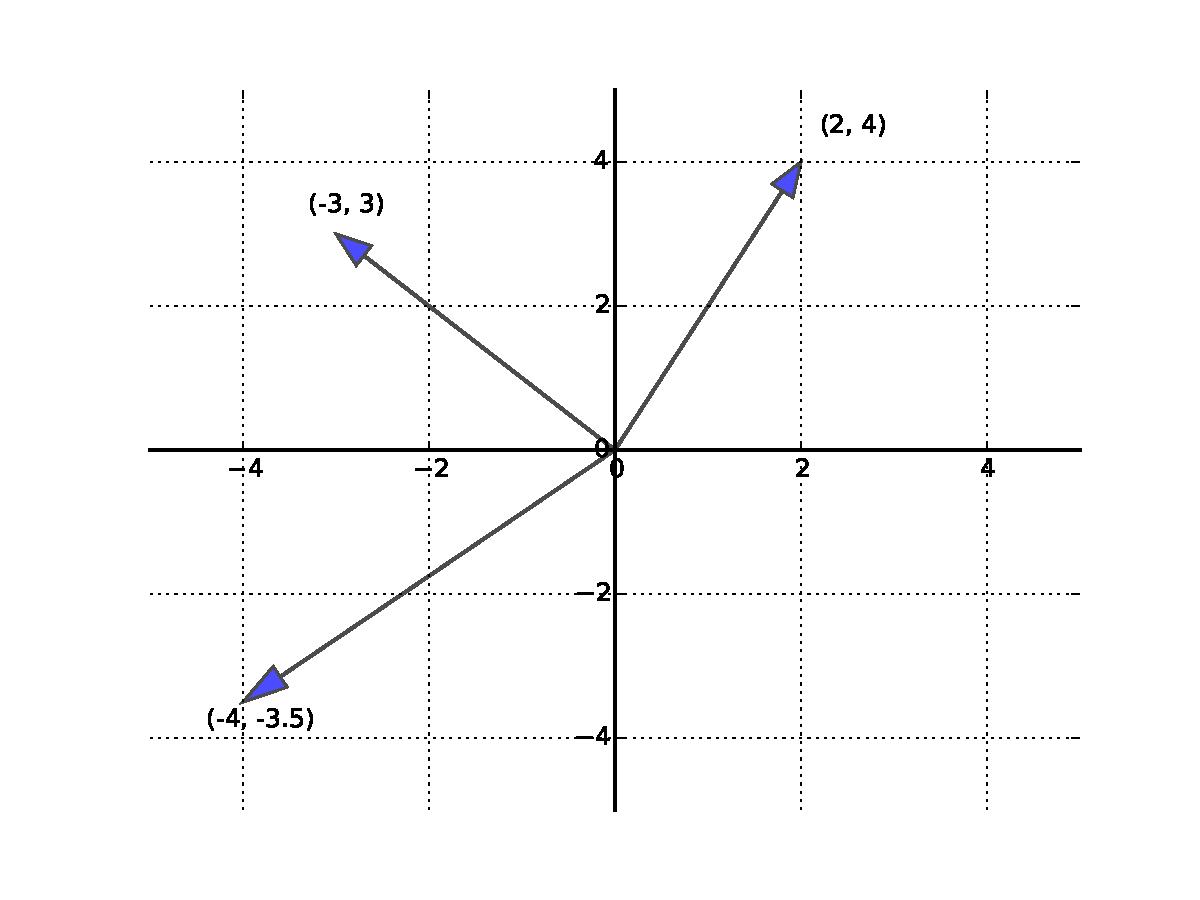
\includegraphics{vecs.pdf}}
       \end{center}
    \end{figure}
    
\end{frame}

\begin{frame}

    \vspace{2em}
    \Eg
    Плоскость
        $P := \setntn{(x_1, x_2, 0) \in \RR^3}{ x_1, x_2 \in \RR}$
    из примера~\ref{ET-eg:planein3d} в ET может быть образована двумя векторами
    
    По теореме~\ref{ET-t:exth}, три вектора на рисунке ниже линейно независимы 
    %
    \begin{figure}
       \begin{center}
           \scalebox{.4}{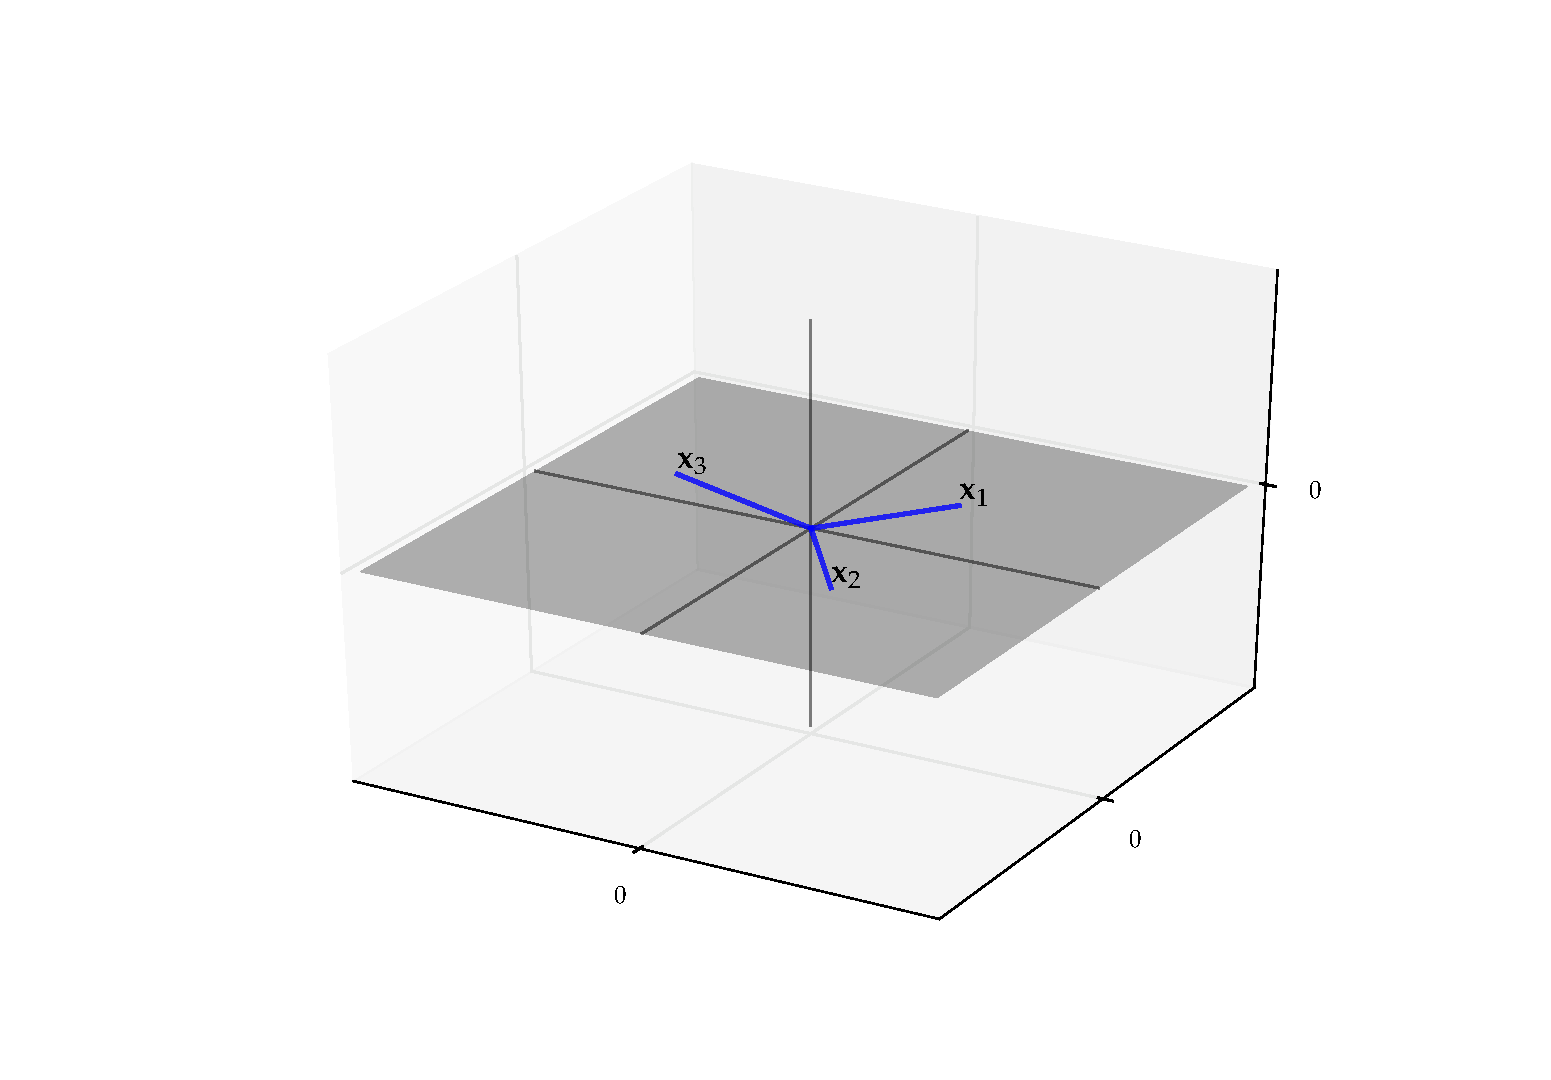
\includegraphics[trim={0 5em 0 15em}, clip]{flat_plane.pdf}}
       \end{center}
    \end{figure}

\end{frame}

\begin{frame}\frametitle{Базисы и размерность}

    \vspace{2em}
    \Thm\eqref{ET-t:bsili}
        Пусть $X := \{ \boldx_1, \ldots, \boldx_N \}$ --- некие $N$ векторов в $\RR^N$.
        Следующие утверждения эквивалентны:
        %
        \begin{enumerate}
            \item $\Span X = \RR^N$
            \item $X$ линейно независим
        \end{enumerate}
    
    \vspace{.7em}
    Для доказательства смотрите~\pageref{ET-t:bsili} в ET
    
\end{frame}

\begin{frame}

    \vspace{2em}
    Пусть $S$ --- линейное подпространство $\RR^N$ и $B \subset S$
    
    \vspace{.7em}
    Множество $B$ называется \navy{базисом} $S$, если
    %
    \begin{enumerate}
        \item $B$ охватывает $S$ и
        \item $B$ линейно независимо
    \end{enumerate}
    
    \vspace{.7em}
    
\end{frame}

\begin{frame}
    
    \vspace{2em}
    Из Теоремы~\ref{ET-t:unor}, когда
    $B$ является базисом $S$, каждая точка $S$ имеет ровно представление
    как линейной комбинации элементов $B$
    
    \vspace{.7em}
    Из Теоремы~\ref{ET-t:bsili}, любые $N$ линейно
    независимых векторов в $\RR^N$ формируют базис в $\RR^N$
    
\end{frame}

\begin{frame}
    
    \vspace{2em}
    \Eg
    Вспомним плоскость из примера выше 
    %
    \begin{equation*}
        P := \setntn{(x_1, x_2, 0) \in \RR^3}{ x_1, x_2 \in \RR}
    \end{equation*}
    %
    Мы показали, что $\Span\{\bolde_1, \bolde_2\} = P$ для 
    %
    \begin{equation*}
        \bolde_1 := 
        \left(
        \begin{array}{c}
            1 \\
            0 \\
            0
        \end{array}
        \right),
        \quad 
        \bolde_2 := 
        \left(
        \begin{array}{c}
            0 \\
            1 \\
            0
        \end{array}
        \right)
    \end{equation*}
    %
    
    Более того, $\{\bolde_1, \bolde_2\}$ линейно независимы (почему?)

    Значит, $\{\bolde_1, \bolde_2\}$ являются базисом для $P$


\end{frame}

\begin{frame}

    \vspace{2em}
    \Thm{\eqref{ET-t:basis}}
    Если $S$ --- линейное подпространство $\RR^N$ отличное от $\{\boldzero\}$, тогда 
    %
    \begin{enumerate}
        \item $S$ имеет по меньшей мере один базис и
        \item каждый базис $S$ имеет одинаковое количество элементов.
    \end{enumerate}
    %
    Если $S$ --- линейное подпространство $\RR^N$, то обычное число, 
    определенное в Теореме~\ref{ET-t:basis} называется \navy{размерностью} $S$,
    и обозначается $\dim S$
    
\end{frame}

\begin{frame}
    
    \vspace{2em}
    \Eg
    Для $P := \setntn{(x_1, x_2, 0) \in \RR^3}{ x_1, x_2 \in \RR}$, $\dim P = 2$, 
    потому что
    %
    \begin{equation*}
        \bolde_1 := 
        \left(
        \begin{array}{c}
            1 \\
            0 \\
            0
        \end{array}
        \right),
        \quad 
        \bolde_2 := 
        \left(
        \begin{array}{c}
            0 \\
            1 \\
            0
        \end{array}
        \right)
    \end{equation*}
    %
    базис имеет два элемента
    
    \vspace{.7em}
    \Eg
    Прямая $\setntn{\alpha \boldx \in \RR^N}{\alpha \in \RR}$, проходящая через начало координат, имеет размерность $1$
    
\end{frame}

\begin{frame}

    \vspace{2em}
    Говорят, что в $\RR^N$ одноэлементное подпространство $\{\boldzero\}$ имеет 
    нулевую размерность
    
    Возьмем множество из $K$ векторов, насколько большой будет его 
    линейная оболочка с точки зрения размерности?  
    
    \vspace{.7em}
    \Thm\eqref{ET-t:dimspan}
        Если $X := \{\boldx_1,\ldots,\boldx_K\} \subset \RR^N$, то
        %
        \begin{enumerate}
            \item $\dim \Span X \leq K$ и
            \item $\dim \Span X = K$ тогда и только тогда, когда $X$ линейно независим
        \end{enumerate}
        %
    Для доказательства смотрите упражнение~\ref{ET-ex:dimspan} в ET
    
\end{frame}

\begin{frame}

    \vspace{2em}
    \Fact{\eqref{ET-fa:ondsrn}}
        Следующие утверждения верны:
        %
        \begin{enumerate}
            \item Пусть $S$ и $S'$ являются линейными подпространствами $\RR^N$ 
            размерности $K$. Если $S \subset S'$, то $S = S'$
            \item Если $S$ --- линейное подпространство $\RR^N$ размерности $M$ и $M < N$, 
            то $S \not= \RR^N$
        \end{enumerate}
        %
        
\end{frame}



\begin{frame}\frametitle{Линейные отображения}

    \vspace{2em}
    Функция $T \colon \RR^K \to \RR^N$ называется
    \navy{линейной}, если 
    %
    \begin{equation*}
            T(\alpha \boldx + \beta \boldy) = \alpha T\boldx + \beta T\boldy
            \qquad
            \forall \, 
            \boldx, \boldy \in \RR^K, \;
            \forall \,
            \alpha, \beta \in \RR
    \end{equation*}
    %

    \vspace{.7em}
    
    Примечание: 
    
    \begin{itemize}
        \item Линейные функции обычно записываются с большой буквы
            \vspace{0.5em}
        \item Обычно, когда это удобно, аргументы в скобках опускаются
    \end{itemize}

\end{frame}

\begin{frame}

    \vspace{2em}
   \Eg Функция $T \colon \RR \to \RR$, определяемая как $Tx = 2x$, линейна 

    Чтобы увидеть это, возьмем любые $\alpha, \beta, x, y$ в $\RR$, тогда 
    %
    \begin{equation*}
      T(\alpha x + \beta y)
      = 2(\alpha x + \beta y)
      = \alpha 2 x + \beta 2 y
      = \alpha Tx + \beta Ty  
    \end{equation*}

    \vspace{.7em}
    \Eg Функция $f \colon \RR \to \RR$, определяемая как $f(x) = x^2$, \underline{не}линейна
    
    Чтобы увидеть это, возьмем $\alpha = \beta = x = y = 1$, получается
    %
    $$f(\alpha x + \beta y) = f(2) = 4$$
    %
    Тем не менее, $\alpha f(x) + \beta f(y) = 1 + 1 = 2$
    
\end{frame}

\begin{frame}
    
    \vspace{2em}
    Примечание: Неправильно думать о линейных функциях как о тех, 
    чей график является прямой
    
    \vspace{.7em}
    \Eg    
    Функция $f \colon \RR \to \RR$, определяемая $f(x) = 1 + 2x$,
    \underline{не}линейна

    Возьмем $\alpha = \beta = x = y = 1$. Имеется
    %
    $$f(\alpha x + \beta y) = f(2) = 5$$
    
    Тем не менее, $\alpha f(x) + \beta f(y) = 3 + 3 = 6$
   
    \vspace{.7em}
    
    Такой вид функции называется \navy{афинной} функцией

\end{frame}

\begin{frame}

    \vspace{2em}
    По определению, если $T$ линейна, то изменение порядка в  
    %
    \[T [ \sum_{k=1}^K \alpha_k \boldx_k ]
    = \sum_{k=1}^K \alpha_k T \boldx_k\]
    %
    будет действительным пока $K=2$
    
    \vspace{.7em}
    Индукция расширяет это до произвольных $K$
    
\end{frame}

\begin{frame}

    \vspace{2em}
    \Fact{\eqref{ET-fa:res}}
    Если $T \colon \RR^K \to \RR^N$ является линейным отображением, то 
    %
    \begin{equation*}
        \range(T) = \Span(V) 
        \quad \text{, где} \quad
        V := \{T\bolde_1, \ldots, T\bolde_K\}
    \end{equation*}


    где $\bolde_k$ является $k$-ым базисным вектором в $\RR^K$
    \vspace{1em}

    \Prf Любой $\boldx \in \RR^K$ может быть выражен как $\sum_{k=1}^K \alpha_k \bolde_k$. 
    Значит, $\range(T)$ является множеством всех точек следующей формы
    %
    \begin{equation*}
        T\boldx 
        = T \left[ \sum_{k=1}^K \alpha_k \bolde_k \right]
        = \sum_{k=1}^K \alpha_k T \bolde_k 
    \end{equation*}
    %
    так как $\alpha_1, \ldots, \alpha_K$ меняется для всех комбинаций.
    Это совпадает с определением $\Span(V)$

\end{frame}

\begin{frame}
    
    \vspace{2em}
    \navy{Ядром} линейного отображения $T \colon \RR^K \to
    \RR^N$ называют
    %
    \begin{equation*}
        \kernel(T) := \setntn{\boldx \in \RR^K}{T\boldx = \boldzero}
    \end{equation*}
    %

    \vspace{.7em}
    \Fact{\eqref{ET-fa:res}}
    Если $T \colon \RR^K \to \RR^N$ линейное отображение, то 
    %
    \begin{equation*}
        \range T = \Span V,
        \quad \text{где } 
        V := \{T\bolde_1, \ldots, T\bolde_K\}
    \end{equation*}
    %
    Доказательства простые (выполните в качестве упражнения)
    
\end{frame}

\begin{frame}
    
    \frametitle{Линейная независимость и биекция}

    \vspace{.7em}
    Много научных и практических задач являются задачами 'обратными'

    \begin{itemize}
        \item мы наблюдаем результаты, но не их причины
        \item как можно работать в обратном порядке, от результатов к причинам?
    \end{itemize}
    
    Примеры

    \begin{itemize}
        \item какие предпочтения потребителей привели к наблюдаемому рыночному поведению?
        \item какие ожидания привели к данному сдвигу обменных курсов?
    \end{itemize}

\end{frame}

\begin{frame}
    
    \vspace{2em}
    В общем, обратную задачу можно выразить как
    
    \begin{figure}
       \begin{center}
        \scalebox{.5}{\input{figs_code/inverse_prob.pdf_t}}
       \end{center}
    \end{figure}

    \begin{itemize}
        \item имеет ли эта задача решение?
        \item является ли оно едиственным?
    \end{itemize}

    Ответы зависят от того, является ли $F$ сюръекцией, инъекцией и т.д. 

    Лучший вариант --- биекция

    Но возникают и другие ситуации

\end{frame}

\begin{frame}

    \vspace{2em}
    \Thm {\eqref{ET-t:linfunc}}
        Если $T$ --- линейная функция из $\RR^N$ в $\RR^N$, то 
        все следующие утверждения эквивалентны:
        %
        \begin{enumerate}
            \item $T$ является биекцией.
            \item $T$ является сюръекцией.
            \item $T$ является инъекцией.
            \item $\kernel T = \{ \boldzero \}$.
            \item $V := \{T\bolde_1, \ldots, T\bolde_N\}$ линейно независимо.
            \item $V := \{T\bolde_1, \ldots, T\bolde_N\}$ формирует базис $\RR^N$.
        \end{enumerate}
        % 
    Смотрите упражнение \ref{ET-ex:linfunc} в ET для доказательства
    
    \vspace{.7em}
    Если любое из этих условий выполняется, то $T$ называют
    \navy{несингулярной}. В ином случае $T$ назвают \navy{сингулярной}
    
\end{frame}

\begin{frame}

    \begin{figure}
       \begin{center}
        \scalebox{.4}{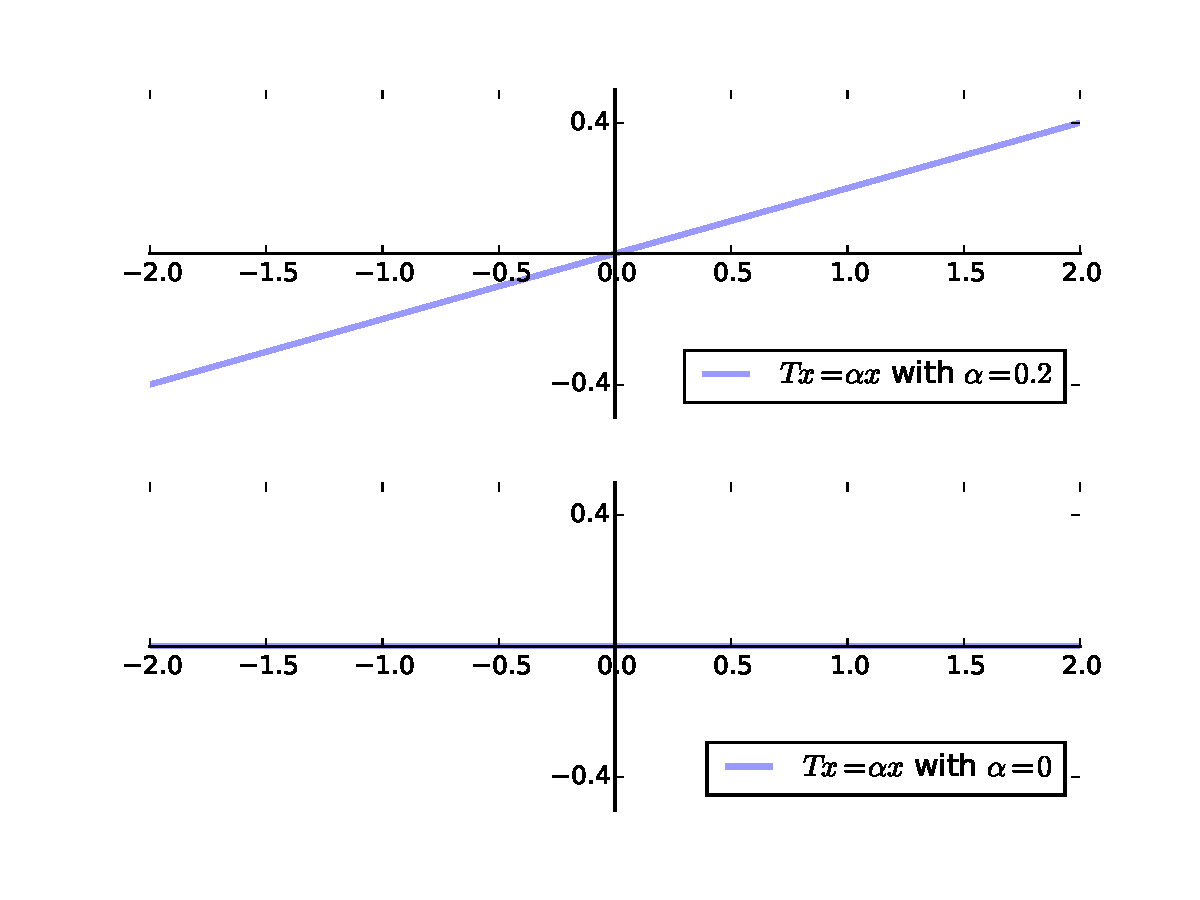
\includegraphics{linbijec.pdf}}
        \caption{Случай с $N=1$, несингулярная и сингулярная функции}
       \end{center}
    \end{figure}
    
\end{frame}

\begin{frame}
    
    \vspace{2em}
    Если $T$ несингулярна, то, будучи биекцией, она должна иметь обратную
    функцию $T^{-1}$, которая так же является биекцией (факт~\ref{ET-fa:bij} на
    странице~\pageref{ET-fa:bij})

    \vspace{.7em}
    \Fact{\eqref{ET-fa:nsins}}
        Если $T \colon \RR^N \to \RR^N$ несингулярна, то и $T^{-1}$ несингулярна.  

    Для доказательства, смотрите упр.~\ref{ET-ex:nsins}
    
\end{frame}

\begin{frame}

    \frametitle{Отображения при различных размерностях} 

    \vspace{2em}
    Помните, что результаты выше применимы к отображениям из $\RR^N$ в $\RR^N$

    Все меняется, когда мы смотрим на линейные отображения при различных размерностях

    \vspace{.7em}

    Общие правили для линейных отображений: 

    \begin{itemize}
        \item отображения из меньших в большие размерности не могут быть сюръекцией
        \item отображения из больших в меньшие размерности не могут быть инъекцией
    \end{itemize}

    Ни один из случаев не может быть биекцией

    \vspace{1em}

\end{frame}

\begin{frame}
    
    \vspace{2em}
    \Thm{\eqref{ET-t:lfoc}}
    Для линейного отображения $T$ из $\RR^K \to \RR^N$, следующие утверждения верны:
    %
    \begin{enumerate}
        \item Если $K < N$, то $T$ не сюръекция.
        \item Если $K > N$, то $T$ не инъекция.
    \end{enumerate}
    %
    \Prf(часть 1)
    
    Пусть $K < N$ и отображение $T \colon \RR^K \to \RR^N$ линейное  
    
    Пусть $V := \{T\bolde_1, \ldots, T\bolde_K\}$, имеется
    %
    $$
    \dim(\range(T)) = \dim(\Span(V)) \leq K < N
    $$
    %
    $$
    \fore 
        \range(T) \not= \RR^N
    $$
    Значит, $T$ не сюръекция 
    
\end{frame}

\begin{frame}
    
    \Prf(часть 2)
    
    Предположим обратное, что $T$ является инъекцией

    Пусть $\alpha_1, \ldots, \alpha_K$ набор векторов, такой что 
    %
    \[
    \alpha_1 T \bolde_1 + \cdots + \alpha_K T \bolde_K = \boldzero
    \]
    %
    \[
    \fore 
    T (\alpha_1 \bolde_1 + \cdots + \alpha_K \bolde_K) = \boldzero
    \qquad (\text{по линейности})
    \]
    %
    \[
    \fore
    \alpha_1 \bolde_1 + \cdots + \alpha_K \bolde_K = \boldzero
    \qquad (\text{так как $\ker(T) = \{\boldzero\}$})
    \]
    %
    \[
    \fore 
    \alpha_1 = \cdots = \alpha_K = 0
    \qquad (\text{по независимости $\{\bolde_1, \ldots \bolde_K\}$)}
    \]

    Мы показали, что $\{T\bolde_1, \ldots, T\bolde_K\}$ линейно независимы

    Но тогда $\RR^N$ содержит линейно независимое множество
    с $K > N$ векторами --- противоречие

\end{frame}


\begin{frame}
    
    \begin{figure}
       \begin{center}
           \scalebox{.4}{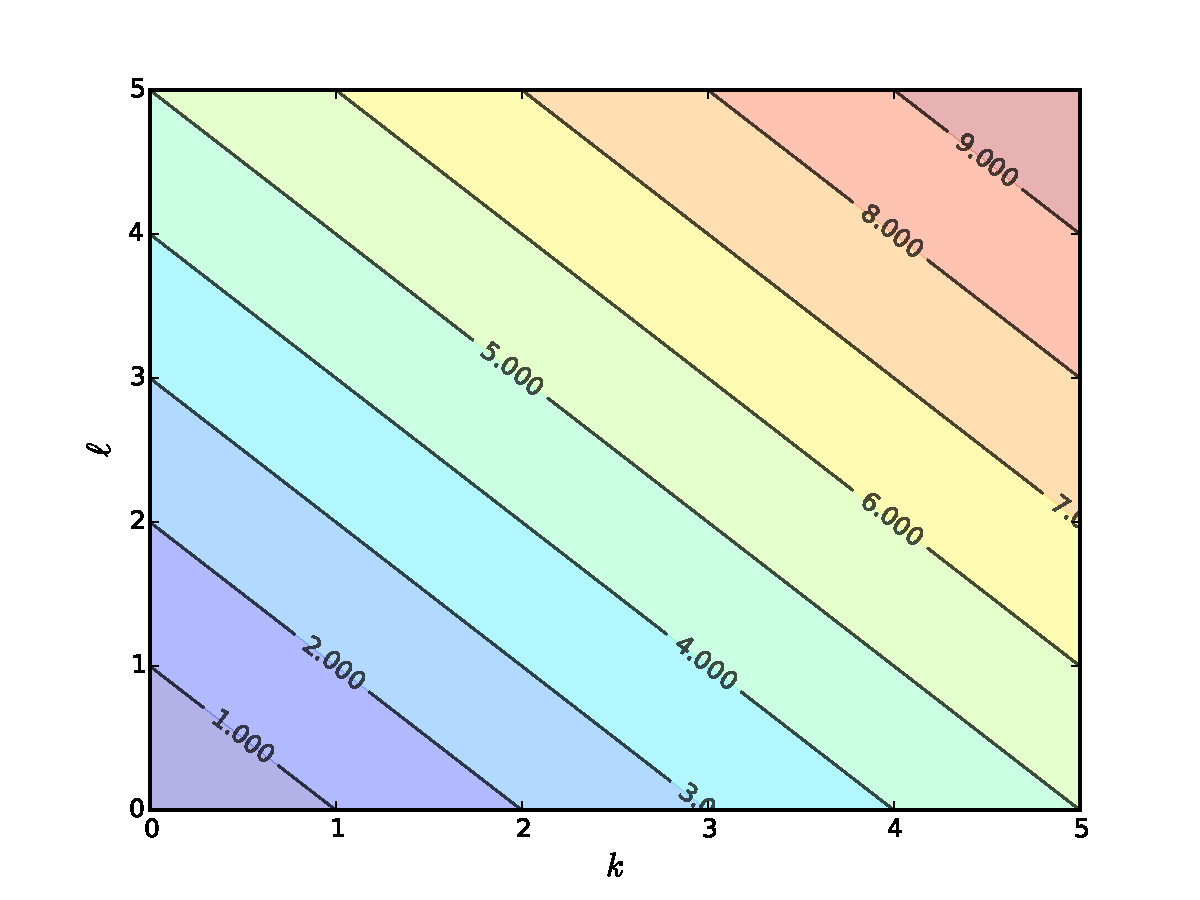
\includegraphics{cost_min_2.pdf}}
       \end{center}
    \end{figure}

   \Eg Функция издержек $c(k, \ell) = rk + w\ell$ не может быть инъекцией

\end{frame}

\begin{frame}\frametitle{Ортогональные векторы и проекции}
    
    \vspace{2em}
    Ключевой концепцией курса является ортогональность -- не только векторов,
    но и случайных величин 
    
    \vspace{.7em}
    Пусть $\boldx$ и $\boldz$ векторы в $\RR^N$
    
    Если $\inner{\boldx,  \boldz} = 0$,
    то мы называем $\boldx$ и $\boldz$ \navy{ортогональными}
    
    Записывается \navy{$\boldx \perp \boldz$}
    
    В $\RR^2$ ортогональный значит перпендикулярный 
    
\end{frame}

\begin{frame}

    \begin{figure}
       \begin{center}
        \begin{tikzpicture}[
    scale=5,
    axis/.style={<->, >=stealth'},
    important line/.style={thick},
    dotted line/.style={dotted, thick,red},
    every node/.style={color=black}
    ]

    % define x,z
    \coordinate(O) at (0,0);
    \coordinate (X) at (-0.2,0.3);
    \coordinate (Z) at (0.6,0.3);
    % axis
    \draw[axis] (-0.4,0)  -- (0.9,0) node(xline)[right] {};
    \draw[axis] (0,-0.3) -- (0,0.7) node(yline)[above] {};
    % x, z
    \draw[important line,blue, ->]  (O) -- (X) node[left] {$\boldx$};
    \draw[important line,blue, ->]  (O) -- (Z) node[right] {$\boldz$};
    % label angle
    \draw[dotted line] (-0.03,0.045) -- (0.03,0.075);
    \draw[dotted line] (0.06,0.03) -- (0.03,0.075);
\end{tikzpicture}

        \caption{\label{f:xpz} $\boldx \perp \boldz$}
       \end{center}
    \end{figure}

\end{frame}

\begin{frame}

     \vspace{2em}
    Пусть $S$ линейное подпространство
    
    \vspace{.7em}
    Говорят, что 
    \navy{$\boldx$ ортогонален $S$}, если $\boldx \perp \boldz$ для всех 
    $\boldz \in S$

    Записывается \navy{$\boldx \perp S$}
    
\end{frame}


\begin{frame}
    
    \begin{figure}
       \begin{center}
        \begin{tikzpicture}[
    scale=5,
    axis/.style={<->, >=stealth'},
    important line/.style={thick},
    dotted line/.style={dotted, thick,red},
    every node/.style={color=black}
    ]

    % define x,z
    \coordinate(O) at (0,0);
    \coordinate (X) at (-0.2,0.3);
    \coordinate (Z1) at (-0.3,-0.15);
    \coordinate (Z2) at (0.8,0.4);
    % axis
    \draw[axis] (-0.4,0)  -- (0.9,0) node(xline)[right] {};
    \draw[axis] (0,-0.3) -- (0,0.7) node(yline)[above] {};
    % x, z
    \draw[important line,blue, ->]  (O) -- (X) node[left] {$\boldx$};
    \draw[important line]  (Z1) -- (Z2) node[right] {$S$};
    % label angle
    \draw[dotted line] (-0.03,0.045) -- (0.03,0.075);
    \draw[dotted line] (0.06,0.03) -- (0.03,0.075);
\end{tikzpicture}

        \caption{\label{f:xpS} $\boldx \perp S$}
       \end{center}
    \end{figure}

\end{frame}

\begin{frame}

    \vspace{2em}
    \Fact\eqref{ET-fa:pythag}
        (Теорема Пифагора)
        
        Если $\{\boldz_1,\ldots, \boldz_K\}$ является ортогональным множеством, то
        %
        \begin{equation*}
            \| \boldz_1 + \cdots + \boldz_K \|^2 
            = \| \boldz_1 \|^2 + \cdots + \| \boldz_K \|^2 
        \end{equation*}
        %
    Докажите в качестве упражнения 
    
    \vspace{.7em}
    \Fact\eqref{ET-fa:orthii}
    Если $O \subset \RR^N$ является ортогональным множеством и $\boldzero \notin O$, то
    $O$ линейно независимо
    
\end{frame}

\begin{frame}
    
    \vspace{2em}
    Ортогональной множество $O \subset \RR^N$ называется \navy{ортонормальное множество} 
    Если $\|\boldu \| = 1$ для всех $\boldu \in O$

    Ортонормальное множество, охватывающее линейное подпространство
    $S$ в $\RR^N$ называют \navy{ортонормальным базисом} $S$
    
    \begin{itemize}
        \item примером ортонормального базиса для всего в $\RR^N$ является
        канонический базис $\{\bolde_1, \ldots, \bolde_N\}$
    \end{itemize}
    
    \vspace{1em}
    \Fact\eqref{ET-fa:bdons}
    Если $\{\boldu_1, \ldots, \boldu_K\}$ является ортонормальным множеством
    и $\boldx \in \Span\{\boldu_1, \ldots, \boldu_K\}$, то
    %
    \begin{equation*}
        \label{eq:exbyob}
        \boldx = \sum_{k=1}^K \inner{\boldx, \boldu_k} \boldu_k
    \end{equation*}
    %
\end{frame}

\section{Ортогональность}

\begin{frame}
    
    \vspace{2em}
    Возьмем $S \subset \RR^N$, \navy{ортогональное дополнение}
    $S$ будет
    %
    \begin{equation*}
        S^{\perp} := \setntn{\boldx \in \RR^N}{\boldx \perp S}
    \end{equation*}
    
    \vspace{.5em}
    \Fact\eqref{ET-fa:ocls}
    Для любого непустого $S \subset \RR^N$, пространство $S^{\perp}$ является
    линейным подпространством $\RR^N$
    
    \Prf 
    Если $\boldx, \boldy \in S^{\perp}$ и $\alpha, \beta \in \RR$, то 
    $\alpha \boldx + \beta \boldy \in S^{\perp}$, 
    так как для любых $\boldz \in S$
    %
    \begin{equation*}
        \inner{\alpha \boldx + \beta \boldy, \boldz}
         = \alpha \inner{ \boldx, \boldz} + \beta \inner{\boldy, \boldz}
         = \alpha \times 0  + \beta \times 0 
         = 0
    \end{equation*}
    
    \vspace{.5em}
    \Fact{\eqref{ET-fa:scscez}}
    Для $S \subset \RR^N$, выполняется $S \cap S^{\perp} =
    \{\boldzero\}$
    
\end{frame}
   
\begin{frame}

    \vspace{2em}
    \begin{figure}
       \begin{center}
        \resizebox{7.5cm}{!}{\begin{tikzpicture}[
    scale=5,
    axis/.style={<->, >=stealth'},
    important line/.style={thick},
    dotted line/.style={dotted, thick,red},
    dashed line/.style={dashed, thin},
    every node/.style={color=black}
    ]

    % define x,z
    \coordinate(O) at (0,0);
    \coordinate (S1) at (-0.4,-0.2);
    \coordinate (S2) at (0.8,0.4);
    \coordinate (S3) at (-0.25,0.5);
    \coordinate (S4) at (0.12,-0.24); 
    % axis
    \draw[axis] (-0.5,0)  -- (0.9,0) node(xline)[right] {};
    \draw[axis] (0,-0.3) -- (0,0.7) node(yline)[above] {};
    % x, z
    \draw[important line, thick]  (S1) -- (S2) node[right] {$S$};
    \draw[important line, thick]  (S4) -- (S3) node[left] {$S^{\perp}$};
    % label angle
    \draw[dotted line] (-0.03,0.06) -- (0.03,0.09);
    \draw[dotted line] (0.06,0.03) -- (0.03,0.09);
   
\end{tikzpicture}
}
        \caption{\label{f:orth_comp} Ортогональное дополнение $S$ в $\mathbb{R}^{2}$}
       \end{center}
    \end{figure}
    
\end{frame}

\begin{frame}\frametitle{Теорема ортогональной проекции}
    
    \vspace{2em}
    Задача:
    %
    \begin{center}
        При данном $\boldy \in \RR^N$ и подпространстве $S$, 
        найти ближайший элемент $S$ к $\boldy$
    \end{center}
    
    Формально: Решаем
    %
    \begin{equation}\label{eq:mproj}
        \hboldy := \argmin_{\boldz \in S} \|\boldy - \boldz\|
    \end{equation}
    %
    Существование, единственность решения не очевидны

    Теорема ортогональной проекции: $\hboldy$ всегда существует, 
    причем в единственном числе

    Также дает полезную характеристику

\end{frame}

\begin{frame}
    
     \vspace{2em}
    \Thm\eqref{ET-t:opt}
    [Теорема ортогональной проекции I]
    
    Пусть $\boldy \in \RR^N$ и $S$ является непустым линейным подпространством в $\RR^N$. 
    
    Следующие утверждения верны:
    %
    \begin{enumerate}
        \item  Задача оптимизации \eqref{eq:mproj} имеет ровно одно решение
        \item $\hboldy \in \RR^N$ является решением \eqref{eq:mproj}
            тогда и только тогда, когда $\hat \boldy \in S$ и 
            $\boldy - \hat \boldy \perp S$
    \end{enumerate}
    
    \vspace{.7em}
    Единственное решение $\hboldy$ называется 
    \navy{ортогональной проекцией $\boldy$ на $S$}  

\end{frame}

\begin{frame}

    \vspace{2em}
    \begin{figure}
       \begin{center}
        \begin{tikzpicture}[
    scale=5,
    axis/.style={<->, >=stealth'},
    important line/.style={thick},
    dotted line/.style={dotted, thick,red},
    dashed line/.style={dashed, thin},
    every node/.style={color=black}
    ]

    % define x,z
    \coordinate(O) at (0,0);
    \coordinate (y-yhat) at (-0.2,0.4);
    \coordinate (yhat) at (0.6,0.3);
    \coordinate (y) at (0.4,0.7);
    \coordinate (Z1) at (-0.4,-0.2);
    \coordinate (Z2) at (0.8,0.4);
    % axis
    \draw[axis] (-0.5,0)  -- (0.9,0) node(xline)[right] {};
    \draw[axis] (0,-0.3) -- (0,0.7) node(yline)[above] {};
    % x, z
    \draw[important line,blue,thick, ->]  (O) -- (yhat) node[below] {$\hboldy$};
    \draw[important line,blue, ->]  (O) -- (y-yhat) node[left] {$\boldy - \hboldy$};
    \draw[important line, thick]  (Z1) -- (O) node[right] {};
    \draw[important line, thick]  (yhat) -- (Z2) node[right] {$S$};
    \draw[important line, blue,->]  (O) -- (y) node[right] {$\boldy$};
    % label angle
    \draw[dotted line] (-0.03,0.06) -- (0.03,0.09);
    \draw[dotted line] (0.06,0.03) -- (0.03,0.09);
    \draw[dotted line] (0.54,0.27) -- (0.51,0.33);
    \draw[dotted line] (0.57,0.36) -- (0.51,0.33);
    \draw[dashed line, black] (y) -- (yhat);
    % path
    \draw[-latex, very thin] (0.5,0.4) to [out=210,in=50] (-0.1,0.2);
\end{tikzpicture}

        \caption{\label{f:orth_proj2D0} Ортогональная проекция}
       \end{center}
    \end{figure}

\end{frame}

\begin{frame}

     \vspace{2em}
    \Prf (достаточности 2.)
    
    Пусть $\boldy \in \RR^N$
    и $S$ является линейным подпространством в $\RR^N$
    
    Пусть $\hat \boldy$ --- вектор в 
    $S$, удовлетворяющий условию $\boldy - \hat \boldy \perp S$
    
    Пусть $\boldz$ --- некая точка в $S$. Получается
    %
    \begin{equation*}
    \| \boldy - \boldz \|^2
    = \| (\boldy - \hat \boldy) + (\hat \boldy - \boldz) \|^2
    = \| \boldy - \hat \boldy \|^2  + \| \hat \boldy - \boldz  \|^2
    \end{equation*}
    %
    Второе равенство следует из $\boldy - \hat \boldy \perp S$ и 
    Теоремы Пифагора
    
    \vspace{.7em}
    Так как $\boldz$ был произвольной точкой в $S$,
    получается $\| \boldy - \boldz \| \geq \| \boldy - \hat \boldy \|$
    для всех $\boldz \in S$
    
\end{frame}

\begin{frame}

    \vspace{2em}
    \Eg
    Пусть $\boldy \in \RR^N$ и $\boldone \in \RR^N$ является вектором из единиц
    
    Пусть $S$ является множеством постоянных векторов в $\RR^N$ --- $S$ 
    является линейной оболочкой $\{\boldone\}$
    
    Ортогональная проекция $\boldy$ на $S$ --- это $\hboldy := \bar y
    \boldone$, где $\bar y := \frac{1}{N} \sum_{n=1}^N y_n$
    
    Ясно, что $\hboldy \in S$ 
    
    \vspace{.7em}
    Чтобы показать, что $\boldy -
    \hboldy$ ортогонален к $S$, нужно проверить
    $\inner{\boldy - \hboldy, \boldone} = 0$ (смотрите упр.~\ref{ET-ex:pecb} на
    странице~\pageref{ET-ex:pecb}). Это верно, так как
    %
    \begin{equation*}
        \inner{\boldy - \hboldy, \boldone }
        = \inner{\boldy, \boldone} - \inner{\hboldy, \boldone}
        = \sum_{n=1}^N y_n - \bar y \inner{\boldone, \boldone}
        = 0
    \end{equation*}
    
\end{frame}

\begin{frame}
    
    \vspace{2em}
    Если зафиксировать подпространство $S$, мы получим функциональную связь
    %
    \begin{equation*}
        \boldy \; \mapsto \text{ его ортогональная проекция } \hat \boldy \in S
    \end{equation*}
    %
    Это четко определенная функция из $\RR^N$ в $\RR^N$
    
    \vspace{.7em}
    Функция обычно обозначается как $\boldP$

    \begin{itemize}
        \item $\boldP(\boldy)$ или $\boldP \boldy$ представляет $\hboldy$
    \end{itemize}
    
    $\boldP$ называется \navy{ортогональным проекционным отображением на $S$}, 
    записывается как
    %
    \begin{equation*}
        \boldP = \proj S
    \end{equation*}

\end{frame}

\begin{frame}

     \vspace{2em}
    \begin{figure}
       \begin{center}
        \begin{tikzpicture}[
    scale=5,
    axis/.style={<->, >=stealth'},
    important line/.style={thick},
    dotted line/.style={dotted, thick,red},
    dashed line/.style={dashed, thin},
    every node/.style={color=black}
    ]

    % define x,z
    \coordinate(O) at (0,0);
    \coordinate (y') at (-0.4,0.1);
    \coordinate (Py) at (0.6,0.3);
    \coordinate (y) at (0.4,0.7);
    \coordinate (Z1) at (-0.4,-0.2);
    \coordinate (Z2) at (0.8,0.4);
    \coordinate (Py') at (-0.28,-0.14);
    % axis
    \draw[axis] (-0.5,0)  -- (0.9,0) node(xline)[right] {};
    \draw[axis] (0,-0.3) -- (0,0.7) node(yline)[above] {};
    % x, z
    \draw[important line,blue,thick, ->]  (O) -- (Py) node[anchor = north west, text width=2em] {$\boldP \boldy$};
    \draw[important line,blue, ->]  (O) -- (y') node[left] {$\boldy'$};
    \draw[important line, thick]  (Z1) -- (O) node[right] {};
    \draw[important line, thick]  (Py) -- (Z2) node[right] {$S$};
    \draw[important line, blue,->]  (O) -- (y) node[right] {$\boldy$};
    % label angle
    \draw[dotted line] (0.54,0.27) -- (0.51,0.33);
    \draw[dotted line] (0.57,0.36) -- (0.51,0.33);
    \draw[dotted line] (-0.22,-0.11) -- (-0.25,-0.05);
    \draw[dotted line] (-0.31,-0.08) -- (-0.25,-0.05);
    \draw[dashed line, black] (y) -- (Py);
    \draw[dashed line, black] (y') -- (Py') node[anchor = north west, text width=5em] {$\boldP \boldy'$};
  
\end{tikzpicture}

        \caption{\label{f:orth_proj2Dp} Ортогональная проекция под $\boldP$}
       \end{center}
    \end{figure}
    
\end{frame}

\begin{frame}

    \vspace{2em}
    \Thm{\eqref{ET-t:opt2}}
    [Теорема ортогональной проекции II]
    
    Пусть $S$ является неким линейным подпространством $\RR^N$, и $\boldP = \proj S$.
    Следующие утверждения верны:
    %
    \begin{enumerate}
        \item $\boldP$ --- линейная функция
    \end{enumerate}
    %
    Более того, для любого $\boldy \in \RR^N$, соблюдается
    %
    \begin{enumerate}
        \setcounter{enumi}{1}
        \item $\boldP \boldy \in S$,
        \item $\boldy - \boldP \boldy \perp S$,
        \item $\| \boldy \|^2 = \| \boldP \boldy \|^2 + \| \boldy - \boldP
            \boldy \|^2$,
        \item $\| \boldP \boldy \| \leq \| \boldy \|$,
        \item $\boldP \boldy = \boldy$ тогда и только тогда, когда $\boldy \in S$, и
        \item $\boldP \boldy = \boldzero$ тогда и только тогда, когда $\boldy \in
            S^{\perp}$.
    \end{enumerate}
    %
    Для доказательства смотрите страницу~\pageref{ET-t:opt2} и
    упражнение \ref{ET-ex:prpil}
    
\end{frame}

\begin{frame}

    \vspace{2em}
    Ниже приводится основополагающий результат 
    
    \vspace{.7em}
    \Fact{\eqref{ET-fa:projon}}
    Если $\{\boldu_1, \ldots, \boldu_K\}$ является ортонормальным базисом для $S$, 
    то для каждого $\boldy \in \RR^N$,
    %
    \begin{equation}
        \label{eq:projon}
        \boldP \boldy = \sum_{k=1}^K \inner{\boldy, \boldu_k} \boldu_k
    \end{equation}
    %
\end{frame}

\begin{frame}

    \vspace{2em}
    \Prf 
    Для начала, правая сторона \eqref{eq:projon} находится в $S$, 
    так как это линейная комбинация векторов, охватывающих $S$
    
    Далее, мы знаем, что $\boldy - \boldP \boldy \perp S$ тогда и только тогда, когда 
    $\boldy - \boldP \boldy \perp \boldu_j$ для каждого $\boldu_j$ из 
    множества базисных векторов (упражнение упр.~\ref{ET-ex:pecb})
    
    Дл любого $\boldy - \boldP \boldy \perp \boldu_j$, выполняется слудующее
    %
    \begin{multline*}
        \inner{\boldy - \boldP \boldy, \boldu_j}
        = \inner{\boldy, \boldu_j }
        -  \sum_{k=1}^K \inner{\boldy, \boldu_k} \inner{\boldu_k, \boldu_j}
        \\ = \inner{\boldy, \boldu_j} - \inner{\boldy, \boldu_j }
        = 0
    \end{multline*}
    %
    Это подтверждает, что $\boldy - \boldP \boldy \perp S$ 
    
\end{frame}

\begin{frame}

    \vspace{2em}
    \Fact{\eqref{ET-fa:subsub}}
    Пусть $S_i$ является линейным подпространством $\RR^N$ для $i=1,2$ и $\boldP_i =
    \proj S_i$. Если $S_1 \subset S_2$, то
    %
    \begin{equation*}
        \boldP_1 \boldP_2 \boldy = \boldP_2 \boldP_1 \boldy = \boldP_1 \boldy
        \quad \text{ для всех } \boldy \in \RR^N
    \end{equation*}
    %

\end{frame}

\begin{frame}\frametitle{Остаточная проекция}

    \vspace{2em}
    Спроецируем $\boldy$ на $S$, где $S$ является линейным подпространством $\RR^N$
    \begin{itemize}
    \item Ближайшая точка к $\boldy$ на $S$ --- это $\hboldy := \boldP \boldy$ 
		    , здесь $\boldP = \proj S$
    \item Если $\boldy$ не находится в $S$, ошибка 
    $\boldy - \boldP \boldy$ существует
    \end{itemize}
    
    \vspace{.7em}
    Введем оператор $\boldM$, который берет $\boldy \in \RR^N$
    и возвращает остаток
    \begin{equation}
        \label{eq:ann0}
        \boldM := \boldI - \boldP
    \end{equation}
    %
    где $\boldI$ является тождественным отображением $\RR^N$
    
\end{frame}

\begin{frame}

     \vspace{2em}
    Для любых $\boldy$ выполняется 
    $\boldM \boldy = \boldI \boldy - \boldP \boldy = \boldy - \boldP \boldy$
    
    \vspace{.7em}
    В регрессионном анализе $\boldM$ проявляется как матрица, называемая 'аннигилятором'
    
    \vspace{.7em}
    Мы говорим о $\boldM$ как об \navy{остаточной проекции}
    
\end{frame}

\begin{frame}

     \vspace{2em}
    \Eg
    Вспомним, что проекция
    $\boldy \in \RR^N$ на $\Span\{\boldone\}$ --- это
    $\bar y \boldone$
    
    Остаточная проекция $\boldM_c \boldy := \boldy -
    \bar y \boldone$
    \begin{itemize}
        \item  вектор ошибок, полученный, когда элементы вектора предсказываются 
        его выборочным средним
    \end{itemize}
    
    
\end{frame}

\begin{frame}

    \vspace{2em}
    \Fact{\eqref{ET-fa:opt3}}
    Пусть $S$ является подпространством $\RR^N$, $\boldP = \proj S$, и 
    $\boldM$ является остаточной проекцией, определенной в \eqref{eq:ann0}.  
    Верны следующие утверждения:
    %
    \begin{enumerate}
        \item $\boldM = \proj S^{\perp}$
        \item $\boldy = \boldP \boldy + \boldM \boldy$ для любых $\boldy \in
            \RR^N$
        \item $\boldP \boldy \perp \boldM \boldy$ для любых $\boldy \in \RR^N$
        \item $\boldM \boldy = \boldzero$ тогда и только тогда, когда $\boldy \in S$
        \item $\boldP \circ \boldM = \boldM \circ \boldP = \boldzero$
    \end{enumerate}
    %
\end{frame}

\begin{frame}
    
    \vspace{2em}
    \begin{figure}
       \begin{center}
        \begin{tikzpicture}[
    scale=5,
    axis/.style={<->, >=stealth'},
    important line/.style={thick},
    dotted line/.style={dotted, thick,red},
    dashed line/.style={dashed, thin},
    every node/.style={color=black}
    ]

    % define x,z
    \coordinate(O) at (0,0);
    \coordinate (uhat) at (-0.2,0.4);
    \coordinate (yhat) at (0.6,0.3);
    \coordinate (y) at (0.4,0.7);
    \coordinate (S1) at (-0.4,-0.2);
    \coordinate (S2) at (0.8,0.4);
    \coordinate (S3) at (-0.3,0.6);
    \coordinate (S4) at (0.12,-0.24); 
    % axis
    \draw[axis] (-0.5,0)  -- (0.9,0) node(xline)[right] {};
    \draw[axis] (0,-0.3) -- (0,0.7) node(yline)[above] {};
    % x, z
    \draw[important line,blue,thick, ->]  (O) -- (yhat) node[anchor = north west, text width=4em] {$\boldP \boldy$};
    \draw[important line,blue, ->]  (O) -- (uhat) node[anchor = north east, text width=4em] {$\boldM \boldy$};
    \draw[important line,thick] (uhat) -- (S3) node [anchor = south east, text width=0.5em] {$S^{\perp}$};
    \draw[important line,thick] (O) -- (S4);
    \draw[important line, thick]  (S1) -- (O) node[right] {};
    \draw[important line, thick]  (yhat) -- (S2) node[right] {$S$};
    \draw[important line, blue,->]  (O) -- (y) node[right] {$\boldy$};
    % label angle
    \draw[dotted line] (-0.03,0.06) -- (0.03,0.09);
    \draw[dotted line] (0.06,0.03) -- (0.03,0.09);
    \draw[dotted line] (0.54,0.27) -- (0.51,0.33);
    \draw[dotted line] (0.57,0.36) -- (0.51,0.33);
    \draw[dotted line] (-0.17,0.34) -- (-0.11,0.37);
    \draw[dotted line] (-0.14,0.43) -- (-0.11,0.37);
    
    \draw[dashed line, black] (y) -- (yhat);
    \draw[dashed line, black] (y) -- (uhat);
    
\end{tikzpicture}

        \caption{\label{f:orth_proj2D} Остаточная проекция}
       \end{center}
    \end{figure}
    
\end{frame}


\begin{frame}

    \vspace{2em}
    Если $S_1$ и $S_2$ --- два подпространства $\RR^N$ и $S_1 \subset S_2$, 
    то $S_2^{\perp} \subset S_1^{\perp}$

    Результат факта~\ref{ET-fa:subsub} обратный для $\boldM$
    
    \vspace{.7em}
    \Fact{\eqref{ET-fa:subsub2}}
    Пусть $S_1$ и $S_2$ --- два подпространства $\RR^N$ и 
    $\boldy \in \RR^N$. Пусть $\boldM_1$ и $\boldM_2$ являются проекциями на $S_1^{\perp}$
    и $S_2^{\perp}$ соответственно. Если $S_1 \subset S_2$, то
    %
    \begin{equation*}
        \boldM_1 \boldM_2 \boldy = \boldM_2 \boldM_1 \boldy = \boldM_2 \boldy
    \end{equation*}
        
\end{frame}

\begin{frame}\frametitle{Ортогонализация Грама-Шмидта} 

    \vspace{2em}
    Вспомним, что любое ортогональное множество $\mathbb{R}^{N}$ не 
    содержащее $\textbf{0}$ линейно независимо -- факт~\ref{ET-fa:orthii}
    
    Вот (важное) частично обратное этому утверждению
    
    \vspace{.7em}
    \Thm{\eqref{ET-t:gso}}
    Для каждого линейно независимого множества $\{\boldb_1, \ldots, \boldb_K\} \subset 
    \RR^N$, существует ортонормальное множество 
    $\{\boldu_1, \ldots, \boldu_K\}$, такое что
    
    %
    \begin{equation*}
        \Span \{\boldb_1, \ldots, \boldb_k\}
        = 
        \Span \{\boldu_1, \ldots, \boldu_k\}
        \quad \text{для } \;
        k = 1, \ldots, K
    \end{equation*}
    %
    Формальные доказательства решаются как упражнения~\ref{ET-ex:gsso}~to~\ref{ET-ex:gssth}
    
\end{frame}


\begin{frame}
    
    \vspace{2em}
    Доказательство дает важный алгоритм построения ортонормированного множества $\{\boldu_1, \ldots, \boldu_K\}$
    
    \vspace{1em}
    Первый шаг --- построить ортогональные множества 
    $\{\boldv_1, \ldots, \boldv_k\}$ с линейной оболочкой, идентичной
    $\{\boldb_1, \ldots, \boldb_k\}$ для каджого $k$
    
    Построение
    $\{\boldv_1, \ldots, \boldv_K\}$ использует 
    \navy{ортогонализацию Грама-Шмидта}:
    
    Для каждого $k = 1, \ldots, K$, пусть 
    %
    \begin{enumerate}
        \item $B_k := \Span\{\boldb_1, \ldots, \boldb_k\}$,
        \item $\boldP_k := \proj B_k$ и $\boldM_k := \proj B_k^{\perp}$,
        \item $\boldv_k := \boldM_{k-1} \boldb_k$, где $\boldM_0$ является
            тождественным отображением, и
        \item $V_k := \Span\{\boldv_1, \ldots, \boldv_k\}$.
    \end{enumerate}
    
\end{frame}

\begin{frame}

    \vspace{2em}
    В шаге 3. мы сопоставляем каждый последующий элемент $\boldb_k$ в подпространство, 
    ортогональное подпространству, созданному с помощью $\boldb_1, \ldots, \boldb_{k-1}$
    
    \vspace{.7em}
    В завершение, определим $\boldu_k$ с помощью $\boldu_k :=
    \boldv_k / \| \boldv_k \|$ 
    
    Множество векторов 
    $\{\boldu_1, \ldots, \boldu_k\}$ является ортонормальным с линейной оболочкой,
    равной $V_k$
    
\end{frame}

\end{document}

